\documentclass{book}
\usepackage{a4wide}

%% possible fonts -- in order of preference
%%\usepackage{palatino}
\usepackage{bookman}
%%\usepackage{charter}
%%\usepackage{newcent}
%%\usepackage{times}
%%\usepackage{avant}
%%\usepackage{helvet}
%%\usepackage{sans}
%%\usepackage{chancery}

\usepackage[T1]{fontenc}
\usepackage{setspace}
\usepackage{ifpdf}
\usepackage{makeidx}
\usepackage{longtable}  %% page wrapping table environment
\usepackage{colortbl}   %% colors for tables
\usepackage{fancyvrb}   %% the "Verbatim" environment
\usepackage{fancyhdr}   %% custom headers and footers
\usepackage{multicol}
\usepackage{listings}   %% source code listings with syntax highlight (lstxxx commands)
\usepackage[tight]{shorttoc}   %% for generating a second table of contents, only containing chapter titles
\usepackage{bytefield}  %% for drawing protocol frames
\usepackage{paralist}   %% for compact lists
\usepackage[nottoc]{tocbibind}  %% makes Bibliography and Index show up in TOC
\settocbibname{References}

\setlength{\textwidth}{160mm}
%\setlength{\oddsidemargin}{12.5mm}
%\setlength{\evensidemargin}{12.5mm}
%\setlength{\topmargin}{0mm}
\setlength{\textheight}{220mm}
%\setlength{\parskip}{1ex}
%\setlength{\parindent}{5ex}

\renewcommand{\bottomfraction}{0.9}
\renewcommand{\topfraction}{0.9}
\renewcommand{\floatpagefraction}{0.9}

%% try to cure overfull hboxes
%% \tolerance=500

%% for navigation in dvi files, only needed by old teTeX versions
%%\usepackage{srcltx}

%% try this for spell checking: cat ess2002.tex | ispell -l -t -a | sort | uniq | more

%%
%% The following snippet changes the horizontal spacing between the number and
%% the title in the table of contents.
%%
%% http://tex.stackexchange.com/questions/33841/how-to-modify-the-space-between-the-numbers-and-text-of-sectioning-titles-in-the
%%
\makeatletter
 \renewcommand*\l@section{\@dottedtocline{1}{2em}{3em}}
 \renewcommand*\l@subsection{\@dottedtocline{2}{5em}{4em}}
\renewcommand*\l@chapter[2]{%
  \ifnum \c@tocdepth >\m@ne
    \addpenalty{-\@highpenalty}%
    \vskip 1.0em \@plus\p@
    \setlength\@tempdima{2em}%
    \begingroup
      \parindent \z@ \rightskip \@pnumwidth
      \parfillskip -\@pnumwidth
      \leavevmode \bfseries
      \advance\leftskip\@tempdima
      \hskip -\leftskip
      #1\nobreak\hfil \nobreak\hb@xt@\@pnumwidth{\hss #2}\par
      \penalty\@highpenalty
    \endgroup
  \fi}
\makeatother

%%
%% OMNeT++ logo, use as {\opp}
%%
\makeatletter
%%\DeclareRobustCommand{\omnetpp}{OM\-NeT\kern-.18em++\@}
\DeclareRobustCommand{\omnetpp}{OMNeT++\@}
\makeatother

\newcommand{\opp}{\omnetpp}

%%
%% PDF Header
%%
% note: \ifpdf now comes from the ifpdf package
%\newif\ifpdf
%\ifx\pdfoutput\undefined
%  \pdffalse
%\else
%  \pdfoutput=1
%  \pdftrue
%\fi
%% PDF-Info
\ifpdf
  \usepackage[pdftex]{graphicx}
  \usepackage[plainpages=false,linktocpage,bookmarksnumbered=true,pdftex]{hyperref}   %% automatic hyperlinking
  \pdfcompresslevel=9
  \pdfinfo{/Author (Andras Varga and others)
    /Title (INET Framework Manual)
    /Subject ()
    /Keywords (INET, INETMANET, OMNeT++, manual)}
\else
  \usepackage{graphicx}
  \usepackage[plainpages=false]{hyperref}   %% automatic hyperlinking
\fi

%%
%% Draft conditional to include unfinished parts
%%
\newif\ifdraft
%\draftfalse %% uncomment for final version
\drafttrue %% uncomment for draft version

%%
%% Generate Index
%%
\makeindex


%%
%% Link colors (hyperref package)
%%
\definecolor{MyDarkBlue}{rgb}{0.16,0.16,0.5}
%% XXX the next line apparently screws up all links except in TOC! they'll be colored nicely, but won't work.
%\hypersetup{
%    colorlinks=true,
%    linkcolor=MyDarkBlue,
%    anchorcolor=MyDarkBlue,
%    citecolor=MyDarkBlue,
%    filecolor=MyDarkBlue,
%    menucolor=MyDarkBlue,
%    runcolor=MyDarkBlue,
%    urlcolor=blue,
%}

%%
%% Heading and Footer
%%
\pagestyle{fancy}
\fancyhf{}
\renewcommand{\footrulewidth}{0.5pt}
\renewcommand{\chaptermark}[1]{\markboth{#1}{}}
\lhead{INET Framework Manual -- \leftmark}
\rfoot{\thepage}

%% this is used for chapter start pages
\fancypagestyle{plain}{
    \rfoot{\thepage}
}

%%
%% Use \begin{graybox}...\end{graybox} for notes
%%
\definecolor{MyGray}{rgb}{0.85,0.85,1.0}
\makeatletter\newenvironment{graybox}%
   {\begin{flushright}\begin{lrbox}{\@tempboxa}\begin{minipage}[r]{0.95\textwidth}}%
   {\end{minipage}\end{lrbox}\colorbox{MyGray}{\usebox{\@tempboxa}}\end{flushright}}%
\makeatother


\newenvironment{note}{\begin{graybox}\textbf{NOTE: }}{\end{graybox}}
\newenvironment{warning}{\begin{graybox}\textbf{WARNING: }}{\end{graybox}}
\newenvironment{caution}{\begin{graybox}\textbf{CAUTION: }}{\end{graybox}}
\newenvironment{rationale}{\begin{graybox}\textbf{Rationale: }}{\end{graybox}}
\newenvironment{important}{\begin{graybox}\textbf{IMPORTANT: }}{\end{graybox}}

%%
%% Set up listings package
%%
\lstloadlanguages{C++,make,perl,tcl,XML,R,Matlab}

%% See listings.pdf,pp20
\lstdefinelanguage{NED} {
    morekeywords={allowunconnected,bool,channel,channelinterface,connections,const,
                  default,double,extends,false,for,gates,if,import,index,inout,input,
                  int,like,module,moduleinterface,network,output,package,parameters,
                  property,simple,sizeof,string,submodules,this,true,types,volatile,
                  xml,xmldoc},
    sensitive=true,
    morecomment=[l]{//},
    morestring=[b]",
}
\lstdefinelanguage{MSG} {
    morekeywords={abstract,bool,char,class,cplusplus,double,enum,extends,false,
                  fields,int,long,message,namespace,noncobject,packet,properties,
                  readonly,short,string,struct,true,unsigned},
    sensitive=true,
    morecomment=[l]{//},
    morestring=[b]",
}
\lstdefinelanguage{inifile} {
    morekeywords={},
    sensitive=true,
    morecomment=[l]{\#},
    morestring=[b]",
}
\lstdefinelanguage{pseudocode} {
    morekeywords={if,then,else,otherwise,whenever,while},
    sensitive=true,
    morecomment=[l]{//},
    morestring=[b]",
    mathescape=true,
}

%% thick ruler on the left; also, designate backtick as LaTeX escape character
%% (e.g. \opp needs to be written as `\opp` inside listing blocks)
\lstset{
    escapechar=`,
    basicstyle=\ttfamily,
    showstringspaces=false,
    frame=leftline,
    framesep=10pt,
    framerule=3pt,
    xleftmargin=15pt
}

\definecolor{NEDRulerColor}{rgb}{0.8,1.0,0.8}  % pale green
\definecolor{MSGRulerColor}{rgb}{0.8,1.0,0.8}  % pale green
\definecolor{CPPRulerColor}{rgb}{0.8,0.8,1.0}  % pale blue
\definecolor{IniRulerColor}{rgb}{0.9,0.9,0.2}  % pale yellow
\definecolor{FileListingRulerColor}{rgb}{0.85,0.85,0.85}  % grey
%\definecolor{CommandLineRulerColor}{rgb}{0.9,0.9,0.2}
\definecolor{PseudoCodeRulerColor}{rgb}{0.0,1.0,1.0}  % cyan

%% See listings.pdf,pp39
\lstnewenvironment{ned}
    {\lstset{language=NED,rulecolor=\color{NEDRulerColor}}}
    {}
\lstnewenvironment{msg}
    {\lstset{language=MSG,rulecolor=\color{MSGRulerColor}}}
    {}
\lstnewenvironment{cpp}
    {\lstset{language=C++,rulecolor=\color{CPPRulerColor}}}
    {}
\lstnewenvironment{inifile}
    {\lstset{language=inifile,rulecolor=\color{IniRulerColor}}}
    {}
\lstnewenvironment{filelisting}
    {\lstset{language={},rulecolor=\color{FileListingRulerColor}}}
    {}
\lstnewenvironment{commandline}
    {\lstset{language={},framesep=11pt,framerule=1pt,xleftmargin=16pt}}
    {}
\lstnewenvironment{pseudocode}
    {\lstset{language=pseudocode,rulecolor=\color{PseudoCodeRulerColor}}}
    {}

%%
%% some customization
%%
\setlength{\parindent}{0pt}
\setlength{\parskip}{1ex}

%%
%% Shortcuts
%%
\newcommand{\appendixchapter}{\chapter} %% html converter needs to know which chapters are appendices

\newcommand{\tbf}{\textbf} %% bold faced text
\newcommand{\ttt}{\texttt} %% type writer font text

\newcommand{\tab}{\hspace*{5mm}} %% tabulator settings

\newcommand{\new}{$^{New!}$}
\newcommand{\changed}{$^{Changed!}$}

%% Colordefinition for table header rows (requires package colortbl)
\newcommand{\tabheadcol}{\rowcolor[gray]{0.8}}

%%
%% Module parameters list
%%
\newenvironment{params}{\begin{itemize}}{\end{itemize}}
\newcommand{\param}[2]{\item \fpar{#1}: #2}

%%
%% Function/Class/Macro/Variable/Program/Parameter/Define names
%%
%% Write the names in type writer font and do an index entry
%% Allows word wrap by automatic hyphenation
%%
%% Usage: \ffunc{take()}
%%    or: \ffunc[take()]{take(obj)}
%% the second form uses the bracketed word for the index entry
%%

%% NED type names
\newcommand{\nedtype}[2][\DefaultOpt]{\def\DefaultOpt{#2}%
  \index{#1}%
  \texttt{\hyphenchar\font=`\-\relax#2}}

%% MSG type names
\newcommand{\msgtype}[2][\DefaultOpt]{\def\DefaultOpt{#2}%
  \index{#1}%
  \texttt{\hyphenchar\font=`\-\relax#2}}

%% Function names
\newcommand{\ffunc}[2][\DefaultOpt]{\def\DefaultOpt{#2}%
  \index{#1}%
  \texttt{\hyphenchar\font=`\-\relax#2}}

%% Class names
\newcommand{\cppclass}[2][\DefaultOpt]{\def\DefaultOpt{#2}%
  \index{#1}%
  \texttt{\hyphenchar\font=`\-\relax#2}}

%% Macro names
\newcommand{\fmac}[2][\DefaultOpt]{\def\DefaultOpt{#2}%
  \index{#1}%
  \texttt{\hyphenchar\font=`\-\relax#2}}

%% Variable names
\newcommand{\fvar}[2][\DefaultOpt]{\def\DefaultOpt{#2}%
  \index{#1}%
  \texttt{\hyphenchar\font=`\-\relax#2}}

%% Program names
\newcommand{\fprog}[2][\DefaultOpt]{\def\DefaultOpt{#2}%
  \index{#1}%
  \texttt{\hyphenchar\font=`\-\relax#2}}

%% Parameter names
\newcommand{\fpar}[2][\DefaultOpt]{\def\DefaultOpt{#2}%
  \index{#1}%
  \texttt{\hyphenchar\font=`\-\relax#2}}

%% Defines
\newcommand{\fdef}[2][\DefaultOpt]{\def\DefaultOpt{#2}%
  \index{#1}%
  \texttt{\hyphenchar\font=`\-\relax#2}}

%% NED/MSG properties
\newcommand{\fprop}[2][\DefaultOpt]{\def\DefaultOpt{#2}%
  \index{#1}%
  \texttt{\hyphenchar\font=`\-\relax#2}}

%% Keywords (NED, MSG)
\newcommand{\fkeyword}[2][\DefaultOpt]{\def\DefaultOpt{#2}%
  \index{#1}%
  \textbf{\texttt{\hyphenchar\font=`\-\relax#2}}}

%% Configuration options
\newcommand{\fconfig}[2][\DefaultOpt]{\def\DefaultOpt{#2}%
  \index{#1}%
  \textbf{\texttt{\hyphenchar\font=`\-\relax#2}}}

%% File names
\newcommand{\ffilename}[2][\DefaultOpt]{\def\DefaultOpt{#2}%
  \index{#1}%
  \texttt{\hyphenchar\font=`\-\relax#2}}

%% Signals
\newcommand{\fsignal}[2][\DefaultOpt]{\def\DefaultOpt{#2}%
  \index{#1}%
  \texttt{\hyphenchar\font=`\-\relax#2}}

\newcommand{\fgate}[1]{\texttt{\hyphenchar\font=`\-\relax#1}}

%% do not number subsubsections
%\setcounter{secnumdepth}{4}

% limit the depth of TOC
\setcounter{tocdepth}{2}

%%
%% Start of document
%%
\begin{document}

%% set the image type preference
\DeclareGraphicsExtensions{.pdf,.png}

\pagestyle{empty}
\pagenumbering{roman}

%% %%\begin{figure}[htbp]
%%\begin{center}
%%\includegraphics[width=3.648in, height=0.990in]{figures/usmanFig1}
%%\end{center}
%% %%\end{figure}

%% the following {center} is a trick -- vspace does nothing if there's
%% nothing above it in the page
\begin{center}\end{center}
\vspace{16em}
\hrule
\vspace{2em}
\begin{center}
{\LARGE INET Framework for OMNeT++}\\
\vspace{1em}
{\large Users Manual}\\
\end{center}
\vspace{2em}
\hrule

%\vspace{4em}
%by {\large Andr\'{a}s Varga}
%\vspace{3em}

\vspace{8em}

\begin{center}
% \textit{WORK IN PROGRESS}
\textit{Generated on \today}
\end{center}



%%% Local Variables:
%%% mode: latex
%%% TeX-master: "usman"
%%% End:

\cleardoublepage

%%\setcounter{page}{1}
%\newpage
%%\pagenumbering{roman}

%% \shorttableofcontents{Chapters}{0}
%% \cleardoublepage

\tableofcontents
\cleardoublepage

\pagestyle{fancy}
\pagenumbering{arabic}

\chapter{Introduction}
\label{cha:introduction}


\section{What is INET Framework}

INET Framework contains IPv4, IPv6, TCP, SCTP, UDP protocol implementations,
and several application models. The framework also includes an MPLS model
with RSVP-TE and LDP signalling. Link-layer models are PPP, Ethernet and 802.11.
Static routing can be set up using network autoconfigurators, or one can use
routing protocol implementations. The INET Framework supports wireless and
mobile simulations as well.


\section{Scope of this Manual}

This manual is written for users of INET who intend to extend INET with new 
components, written in C++. This manual is accompanied by the INET Reference,
which is generated from NED and MSG files using OMNeT++'s documentation generator, 
and the documentation of the underlying C++ classes, generated from the source files 
using Doxygen. A working knowledge of OMNeT++ and the C++ language is assumed.

\ifdraft TODO
\section{Contents of this Manual}

todo...
\fi


%%% Local Variables:
%%% mode: latex
%%% TeX-master: "usman"
%%% End:


\cleardoublepage

\chapter{Using the INET Framework}
\label{cha:usage}

\section{Installation}

To install the INET Framework, download the most recent INET Framework source
release from the download link on the http://inet.omnetpp.org web site,
unpack it, and follow the instructions in the INSTALL file in the root
directory of the archive.

\ifdraft TODO
If you plan to simulate ad-hoc networks or you need more wireless link layer
protocols than provided in INET, download and install the INETMANET source
archive instead. (INETMANET aready contains a copy of the INET Framework.)

If you plan to make use of other INET extensions (e.g. HttpTools, VoipTools or TraCI),
follow the installation instructions provided with them. If there are no
install instructions, check if the archive contains a \ttt{.project} file.
If it does, then the project can be imported into the IDE (use File > Import >
General > Existing Project into workspace); make sure that the project is recognized
as an OMNeT++ project (the Project Properties dialog contains an OMNeT++ page)
and it lists the INET or INETMANET project as dependency (check the Project References
page in the Project Properties dialog).

If the extension project contains no \ttt{.project} file, create an empty OMNeT++
project using the New OMNeT++ Project wizard in File > New, add the INET or INETMANET
project as dependency using the Project References page in the Project Properties dialog,
and copy the source files into the project.
\fi

After installation, run the example simulations to make sure everything works
correctly. The INSTALL file also describes how to do that.


\section{INET as an OMNeT++-based simulation framework}

\ifdraft TODO
what is documented where in the OMNeT++ manual (chapter, section title)
\fi

The INET Framework builds upon OMNeT++, and uses the same concept: modules
that communicate by message passing. Hosts, routers, switches and other
network devices are represented by OMNeT++ compound modules. These compound
modules are assembled from simple modules that represent protocols,
applications, and other functional units. A network is again an OMNeT++
compound module that contains host, router and other modules. The external
interfaces of modules are described in NED files. NED files describe the
parameters and gates (i.e. ports or connectors) of modules, and also the
submodules and connections (i.e. netlist) of compound modules.

Modules are organized into hierarchical \textit{packages} that directly map to
a folder tree, very much like Java packages. Packages in
INET are organized roughly according to OSI layers; the top packages
include \ttt{inet.applications}, \ttt{inet.transportlayer},
\ttt{inet.networklayer}, \ttt{inet.linklayer}, and \ttt{inet.physicallayer}. 
Other packages are \ttt{inet.routing}, \ttt{inet.mobility}, \ttt{inet.power}, 
\ttt{inet.environment}, and \ttt{inet.node}. These packages correspond to the
\ttt{src/applications/}, \ttt{src/transportlayer/}, etc. directories in the
INET source tree. (The \ttt{src/inet/} directory corresponds to the \ttt{inet} 
package, as defined by the \ttt{src/inet/package.ned} file.) Subdirectories
within the top packages usually correspond to concrete protocols or protocol
families. The implementations of simple modules are C++ classes with the same
name, with the source files placed in the same directory as the NED file.

The \ttt{inet.node} package contains various pre-assembled host, router,
switch, access point, and other modules, for example
\nedtype{StandardHost}, \nedtype{Router} and \nedtype{EtherSwitch} and
\nedtype{AccessPoint}. These compound modules contain some customization
options via parametric submodule types, but they are not meant to be
universal, so it may be necessary to create your own node models for
your particular simulation scenarios.

Network interfaces (Ethernet, IEEE 802.11, etc) are usually compound modules
themselves, and are being composed of a queue, a MAC, and possibly other
simple modules. See \nedtype{EthernetInterface} as an example.

Not all modules implement protocols. There are modules which hold data (for
example \nedtype{IPv4RoutingTable}), perform autoconfiguration of a network
(\nedtype{IPv4NetworkConfigurator}), move a mobile node around (for example
\nedtype{ConstSpeedMobility}), and perform housekeeping associated with
radio signals in wireless simulations (\nedtype{RadioMedium}).

Protocol headers and packet formats are described in message definition
files (msg files), which are translated into C++ classes by OMNeT++'s
\textit{opp\_msgc} tool. The generated message classes subclass from OMNeT++'s
\ttt{cPacket} or \ttt{cMessage} classes.

The internal structure of compound modules such as host and router models
can be customized in several ways. The first way is the use of \textit{gate
vectors} and \textit{submodule vectors}. The sizes of vectors may come from
parameters or derived by the number of external connections to the module.
For example, one can have an Ethernet switch model that has as many ports
as needed, i.e. equal to the number of Ethernet devices connected to it.

The second way of customization is \textit{parametric types}, that is, the
type of a submodule (or a channel) may be specified as a string parameter.
For example, the relay unit inside an Ethernet switch has several
alternative implementations, each one being a distinct module type. The
switch model contains a parameter which allows the user to select the
appropriate relay unit implementation.

A third way of customizing modules is \textit{inheritance}: a derived
module may add new parameters, gates, submodules or connections, and may
set inherited unassigned parameters to specific values.


\section{Creating and Running Simulations}

To create a simulation, you would write a NED file that contains the network,
i.e. routers, hosts and other network devices connected together. You can
use a text editor or the IDE's graphical editor to create the network.

Modules in the network contain a lot of unassigned parameters, which need
to be assigned before the simulation can be run.\footnote{The simulator can
interactively ask for parameter values, but this is not very convenient
for repeated runs.} The name of the network to be simulated, parameter values
and other configuration option need to be specified in the \ttt{omnetpp.ini}
file.\footnote{This is the default file name; using other is also possible.}

\ttt{omnetpp.ini} contains parameter assignments as \textit{key=value}
lines, where each key is a wildcard pattern. The simulator matches these
wildcard patterns against full path of the parameter in the module tree
(something like \ttt{Test.host[2].tcp.nagleEnabled}), and value from
the first match will be assigned for the parameter. If no matching line is
found, the default value in the NED file will be used. (If there is no
default value either, the value will be interactively prompted for, or, in
case of a batch run, an error will be raised.)

There are two kinds of wildcards: a single asterisk \ttt{*} matches at most
one component name in the path string, while double asterisk \ttt{**} may
match multiple components. Technically: \ttt{*} never matches a dot or a
square bracket (\ttt{.}, \ttt{[}, \ttt{]}), while \ttt{**} can match any of
them. Patterns are also capable of expressing index ranges
(\ttt{**.host[1..3,5,8].tcp.nagleEnabled}) and ranges of numbers embedded
in names (\ttt{**.switch\{2..3\}.relayUnitType}).

OMNeT++ allows several configurations to be put into the \ttt{omnetpp.ini}
file under \ttt{[Config <name>]} section headers, and the right
configuration can be selected via command-line options when the simulation
is run. Configurations can also build on each other: \ttt{extends=<name>}
lines can be used to set up an inheritance tree among them. This feature
allows minimizing clutter in ini files by letting you factor out common
parts. (Another ways of factoring out common parts are ini file inclusion
and specifying multiple ini files to a simulation.) Settings in the
\ttt{[General]} section apply to all configurations, i.e. \ttt{[General]}
is the root of the section inheritance tree.

Parameter studies can be defined by specifying multiple values for a
parameter, with the \ttt{\$\{10,50,100..500 step 100, 1000\}} syntax;
a repeat count can also be specified.

\ifdraft TODO
how to run;

C++ -> dll (opp\_run) or exe
\fi

\ifdraft TODO
\section{Result Collection and Analysis}

how to anaylize results

how to configure result collection
\fi


\ifdraft TODO
\section{TODO}
Some modules have only one instance, at global network level:

\nedtype{IPv4NetworkConfigurator} assigns IP addresses to hosts and routers,
and sets up static routing.

\nedtype{ScenarioManager} makes simulations scriptable. Modules can be made to support
scripting by implementing the \cppclass{IScriptable} C++ interface.
\fi


\section{Setting up wired network simulations}

For an introduction, in this section we show you how to set up simulations
of wired networks using PPP or Ethernet links with autoconfigured static IP
routing. (If your simulation involves more, such as manually configured
routing tables, dynamic routing, MPLS, or IPv6 or other features and protocols,
you'll find info about them in later chapters.)

Such a network can be assembled using the predefined \nedtype{StandardHost}
and \nedtype{Router} modules. For automatic IP address assignment and
static IP routing we can use the \nedtype{IPv4NetworkConfigurator} utility
module.

\ifdraft TODO
ethg, pppg;  automatically expand (++)

todo which modules are needed into it, what they do, etc.

how to add apps, etc
\fi

\ifdraft TODO
\subsection{Modeling Link and Node Failures}

more
\fi


\section{Setting up wireless network simulations}

In this section we show you how to set up wireless network simulations using
IEEE 802.11 links with autoconfigured static IP routing. Such a network can be
assembled using the predefined \nedtype{WirelessHost} and \nedtype{AccessPoint}
modules. \nedtype{RadioMedium} is also required for wireless simulations. It
keeps track of which nodes are within interference distance of other nodes.


\section{Specifying network addresses in module parameters}

In INET, TCP, UDP and all application layer modules work with
both IPv4 and IPv6. Internally they use the \cppclass{L3Address} C++ class, which
can represent both IPv4 and IPv6 addresses.

Most modules use the \cppclass{L3AddressResolver} C++ class to resolve addresses
specified in module parameters in omnetpp.ini.
\cppclass{L3AddressResolver} accepts the following syntax:

\begin{itemize}
  \item literal IPv4 address: \ttt{"186.54.66.2"}
  \item literal IPv6 address: \ttt{"3011:7cd6:750b:5fd6:aba3:c231:e9f9:6a43"}
  \item module name: \ttt{"server"}, \ttt{"subnet.server[3]"}
  \item interface of a host or router: \ttt{"server/eth0"}, \ttt{"subnet.server[3]/eth0"}
  \item IPv4 or IPv6 address of a host or router: \ttt{"server(ipv4)"},
      \ttt{"subnet.server[3](ipv6)"}
  \item IPv4 or IPv6 address of an interface of a host or router:
      \ttt{"server/eth0(ipv4)"}, \ttt{"subnet.server[3]/eth0(ipv6)"}
\end{itemize}


\ifdraft TODO
\section{Setting up ad-hoc network simulations}

todo which modules are needed into it, what they do, etc.
\fi

\ifdraft TODO
\section{Emulation}
\fi

\ifdraft TODO
\section{Packet traces}

Recording packet traces

Traffic generation using packet traces
\fi

\ifdraft TODO
\section{Developing New Protocols}

where to put the source files: you can copy and modify the INET framework (fork it)
in the hope that you'll contribute back the changes; or you can develop in
a separate project (create new project in the IDE; mark INET as referenced project)

NED and source files in the same folder; examples under examples/; etc.

for details, read the OMNeT++ manual and the following chapters of this manual

\fi



%%% Local Variables:
%%% mode: latex
%%% TeX-master: "usman"
%%% End:


\cleardoublepage

\chapter{Node Architecture}
\label{cha:node-architecture}


\section{Overview}

This chapter describes the architecture of INET host and router models.

Hosts and routers in the INET Framework are OMNeT++ compound modules that
are composed of the following ingredients:

\begin{itemize}

\item \tbf{Interface Table (\nedtype{InterfaceTable})}. This module
contains the table of network interfaces (eth0, wlan0, etc) in the host.
Interfaces are registered dynamically during the initialization phase by
modules that represent network interface cards (NICs). Other modules access
interface information via a C++ class interface.

\item \tbf{Routing Table (\nedtype{IPv4RoutingTable})}. This module contains
the IPv4 routing table. It is also accessed from other modules via a C++ interface.
The interface contains member functions for adding, removing, enumerating
and looking up routes, and finding the best matching route for a given
destination IPv4 address. The IPv4 module calls the latter function for
routing packets, and routing protocols such as OSPF or BGP call the route
manipulation methods to add and manage discovered routes. For IPv6
simulations, \nedtype{IPv4RoutingTable} is replaced (or co-exists) with
a \nedtype{IPv6RoutingTable} module, possibly with a \nedtype{BindingCache}
module as well.

\ifdraft TODO
; and for Mobile IPv6 simulations (xMIPv6 project [TODO])
\fi

\ifdraft TODO
\item \tbf{Notification Board (\nedtype{NotificationBoard})}. This module
makes it possible for several modules to communicate in a publish-subscribe
manner. Notifications include change notifications (``routing table
changed'') and state changes (``radio became idle'').
\fi

\item \tbf{Mobility module}. In simulations involving node mobility, this
module is responsible for moving around the node in the simulated
``playground.'' A mobility module is also needed for wireless simulations
even if the node is stationary, because the mobility module stores the
node's location, needed to compute wireless transmissions. Different
mobility models (Random Walk, etc.) are supported via different module
types, and many host models define their mobility submodules with
parametric type so that the mobility model can be changed in the
configuration (\ttt{"mobility: <mobilityType> like IMobility"}).

\item \tbf{NICs}. Network interfaces are usually compound modules
themselves, composed of a queue and a MAC module (and in the case of
wireless NICs, a radio module or modules). Examples are
\nedtype{PPPInterface}, \nedtype{EthernetInterface}, and WLAN interfaces
such as \nedtype{Ieee80211NicSTA}. The queue submodule stores packets
waiting for transmission, and it is usually defined as having parametric
type as it has multiple implementations to accommodate different needs
(\nedtype{DropTailQueue}, \nedtype{REDQueue}, \nedtype{DropTailQoSQueue},
etc.) Most MACs also have an internal queue to allow operation without an
external queue module, the advantage being smaller overhead. The NIC's
entry in the host's \nedtype{InterfaceTable} is usually registered by the
MAC module at the beginning of the simulation.

\item \tbf{Network layer}. Modules that represent protocols of the network
layer are usually grouped into a compound module: \nedtype{IPv4NetworkLayer}
for IPv4, and \nedtype{IPv6NetworkLayer} for IPv6. \nedtype{IPv4NetworkLayer}
contains the modules \nedtype{IPv4}, \nedtype{ARP}, \nedtype{ICMP} and
\nedtype{ErrorHandling}. The \nedtype{IPv4} module performs IP
encapsulation/decapsulation and routing of datagrams; for the latter it
accesses the C++ function call interface of the \nedtype{IPv4RoutingTable}.
Packet forwarding can be turned on/off via a module parameter. The
\nedtype{ARP} module is put into the path of packets leaving the network
layer towards the NICs, and performs address resolution for interfaces that
need it (e.g. Ethernet). \nedtype{ICMP} deals with sending and receiving
ICMP packets. The \nedtype{ErrorHandling} module receives and logs ICMP
error replies. The IPv6 network layer, \nedtype{IPv6NetworkLayer} contains the
modules \nedtype{IPv6}, \nedtype{ICMPv6}, \nedtype{IPv6NeighbourDiscovery}
and \nedtype{IPv6ErrorHandling}. For Mobile IPv6 simulations 

\ifdraft TODO
(xMIPv6 project [TODO]),
\fi

\nedtype{IPv6NetworkLayer} is extended with further modules.

\item \tbf{Transport layer protocols}. Transport protocols are represented
by modules connected to the network layer; currently TCP, UDP and SCTP are
supported. TCP has several implementations: \nedtype{TCP} is the OMNeT++
native implementation; the \nedtype{TCP\_lwip} module wraps the lwIP TCP
stack \ifdraft [TODO] \fi; and the \nedtype{TCP\_NSC} module wraps the Network
Simulation Cradle library \ifdraft [TODO] \fi. For this reason, the \ttt{tcp} 
submodule is usually defined with a parametric submodule type (\ttt{"tcp:
<tcpType> like ITCP"}). UDP and SCTP are implemented by the \nedtype{UDP} and
\nedtype{SCTP} modules, respectively.

\item \sloppypar \tbf{Applications}. Application modules typically connect to TCP
and/or UDP, and model the user behavior as well as the application program
(e.g. browser) and application layer protocol (e.g. HTTP). For convenience,
\nedtype{StandardHost} supports any number of UDP, TCP and SCTP
applications, their types being parametric (\ttt{"tcpApp[numTcpApps]:
<tcpAppType> like TCPApp; udpApp[numUdpApps]: <udpAppType> like
UDPApp; ..."}). This way the user can configure applications entirely from
\ttt{omnetpp.ini}, and does not need to write a new NED file every time
different applications are needed in a host model. Application modules
are typically not present in router models.

\item \tbf{Routing protocols}. Router models typically contain modules that
implement routing protocols such as OSPF or BGP. These modules are
connected to the TCP and/or the UDP module, and manipulate routes in the
\nedtype{IPv4RoutingTable} module via C++ function calls.

\item \tbf{MPLS modules}. Additional modules are needed for MPLS
simulations. The \nedtype{MPLS} module is placed between the network layer
and NICs, and implements label switching. \nedtype{MPLS} requires a
\nedtype{LIB} module (Label Information Base) to be present in the router
which it accesses via C++ function calls. MPLS control protocol
implementations (e.g. the \nedtype{RSVP} module) manage the information in
\nedtype{LIB} via C++ calls.

\item \tbf{Relay unit}. Ethernet (and possibly other) switch models may
contain a relay unit, which switches frames among Ethernet (and other
IEEE 802) NICs. Concrete relay unit types include \nedtype{MACRelayUnit}
and \nedtype{Ieee8021dRelay}, which differ in their performance models.

\ifdraft TODO
\item \tbf{Power consumption}. INET extensions uses for wireless sensor
networks (WSNs) may add a battery module to the node model. The battery
module would keep track of energy consumption. A battery module is provided
e.g. by the INETMANET project.
\fi

\end{itemize}

The \nedtype{StandardHost} and \nedtype{Router} predefined NED types are
only one possible example of host/router models, and they do not contain
all the above components; for specific simulations it is a perfectly
valid approach to create custom node models.

Most modules are optional, i.e. can be left out of hosts or other node
models when not needed in the given scenario. For example, switch models do
not need a network layer, a routing table or interface table. Some NICs (e.g.
\nedtype{EtherMAC}) can be used without and interface table and queue models as
well.

\ifdraft TODO
The notification board (\nedtype{NotificationBoard}) and the interface
table (\nedtype{InterfaceTable}) will be described later in this chapter.
Other modules are covered in later chapters, i.e. \nedtype{IPv4RoutingTable}
in the IPv4 chapter.
\fi





%%% Local Variables:
%%% mode: latex
%%% TeX-master: "usman"
%%% End:


\cleardoublepage

\chapter{Point-to-Point Links}
\label{cha:ppp}


\section{Overview}

The modules of the PPP model can be found in the \nedtype{inet.linklayer.ppp}
package. The \nedtype{PPP} simple module performs encapsulation
of network datagrams into PPP frames and decapsulation of
the incoming PPP frames.

\section{Sending PPP Frames}

TODO how to send; accepted tags; example code

\section{Receiving PPP Frames}

TODO tags PPP attaches to packets; example code

\section{Extending the PPP Module}

TODO how (override handleMessage etc.)

%%% Local Variables:
%%% mode: latex
%%% TeX-master: "usman"
%%% End:



\cleardoublepage

% last synchronized to 'dbc28949bf4332ac86d84b95705fbea9af4f84f7'
\chapter{The Ethernet Model}
\label{cha:ethernet}

\section{Sending Ethernet Frames}

TODO tags etc

\section{Receiving Ethernet Frames}

TODO tags etc

\section{Frames}

The INET defines these frames in the \ffilename{EtherFrame.msg} file.
The models supports Ethernet II, 803.2 with LLC header, and 803.3 with LLC and SNAP headers.
The corresponding classes are:
\msgtype{EthernetIIFrame}, \msgtype{EtherFrameWithLLC} and \msgtype{EtherFrameWithSNAP}. They all class
from \msgtype{EtherFrame} which only represents the basic MAC frame with source and
destination addresses. \nedtype{EtherMAC} only deals with \msgtype{EtherFrame}s, and does not
care about the specific subclass.

Ethernet frames carry data packets as encapsulated cMessage objects.
Data packets can be of any message type (cMessage or cMessage subclass).

The model encapsulates data packets in Ethernet frames using the \ttt{encapsulate()}
method of cMessage. Encapsulate() updates the length of the Ethernet frame too,
so the model doesn't have to take care of that.

The fields of the Ethernet header are passed in a \cppclass{Ieee802Ctrl}
control structure to the LLC by the network layer.


EtherJam, EtherPadding (interframe gap), EtherPauseFrame?


\subsection{EtherLLC}

EtherFrameWithLLC

SAP registration

% TODO delete EtherLLC, because LLC without SNAP is not used with IP (no ARP,IPv6 SAP)
% TODO modify EtherEncap to handle EtherFrameWithSNAP frames too (we can not send EtherFrameWithSNAP now)

\subsubsection{\nedtype{EtherLLC} and higher layers}

The \nedtype{EtherLLC} module can serve several applications (higher layer protocols),
and dispatch data to them. Higher layers are identified by DSAP.
See section "Application registration" for more info.

\nedtype{EtherEncap} doesn't have the functionality to dispatch to different
higher layers because in practice it'll always be used with IP.

\subsubsection{Communication between LLC and Higher Layers}

Higher layers (applications or protocols) talk to the \nedtype{EtherLLC} module.

When a higher layer wants to send a packet via Ethernet, it just
passes the data packet (a cMessage or any subclass) to \nedtype{EtherLLC}.
The message kind has to be set to IEEE802CTRL\_DATA.

In general, if \nedtype{EtherLLC} receives a packet from the higher layers,
it interprets the message kind as a command. The commands include
IEEE802CTRL\_DATA (send a frame), IEEE802CTRL\_REGISTER\_DSAP (register highher layer)
IEEE802CTRL\_DEREGISTER\_DSAP (deregister higher layer) and IEEE802CTRL\_SENDPAUSE
(send PAUSE frame) -- see EtherLLC for a more complete list.

The arguments to the command are NOT inside the data packet but
in a "control info" data structure of class \cppclass{Ieee802Ctrl}, attached to
the packet. See controlInfo() method of cMessage (OMNeT++ 3.0).

For example, to send a packet to a given MAC address and protocol
identifier, the application sets the data packet's message kind
to ETH\_DATA ("please send this data packet" command),
fills in the \nedtype{Ieee802Ctrl} structure with the destination MAC address and
the protocol identifier, adds the control info to the message, then sends
the packet to \nedtype{EtherLLC}.

When the command doesn't involve a data packet (e.g.
IEEE802CTRL\_(DE)REGISTER\_DSAP, IEEE802CTRL\_SENDPAUSE), a dummy packet
(empty cMessage) is used.

\subsubsection{Rationale}

The alternative of the above communications would be:

\begin{itemize}
  \item adding the parameters such as destination address into the data
    packet. This would be a poor solution since it would make the
    higher layers specific to the Ethernet model.
  \item encapsulating a data packet into an \textit{interface packet} which
    contains the destination address and other parameters. The
    disadvantages of this approach is the overhead associated with
    creating and destroying the interface packets.
\end{itemize}

Using a control structure is more efficient than the interface packet
approach, because the control structure can be created once inside
the higher layer and be reused for every packet.

It may also appear to be more intuitive in Tkenv because one can observe
data packets travelling between the higher layer and Ethernet
modules -- as opposed to "interface" packets.


\subsubsection{EtherLLC: SAP Registration}

The Ethernet model supports multiple applications or higher layer
protocols.

So that data arriving from the network can be dispatched to the
correct applications (higher layer protocols), applications
have to register themselves in \nedtype{EtherLLC}. The registration
is done with the IEEE802CTRL\_REGISTER\_DSAP command
(see section "Communication between LLC and higher layers")
which associates a SAP with the LLC port. Different applications
have to connect to different ports of \nedtype{EtherLLC}.

The ETHERCTRL\_REGISTER\_DSAP/IEEE802CTRL\_DEREGISTER\_DSAP commands use only the
dsap field in the \cppclass{Ieee802Ctrl} structure.

%%% Local Variables:
%%% mode: latex
%%% TeX-master: "usman"
%%% End:

\cleardoublepage

\chapter{The Physical Environment}
\label{cha:environment}

TODO C++ interface

%%% Local Variables:
%%% mode: latex
%%% TeX-master: "usman"
%%% End:


\cleardoublepage

\chapter{The Power Model}
\label{cha:power}

\section{Overview}

Modeling power consumption becomes more and more important with the increasing
number of embedded devices and the upcoming Internet of things. Mobile personal
medical devices, large scale wireless environment monitoring devices, electric
vehicles, solar panels, low-power wireless sensors, etc. require paying special
attention to power consumption. The high fidelity simulation of power
consumption allows designing power sensitive routing protocols, MAC protocols,
physical layers, etc. which in turn results in more energy efficient devices.

In order to help the modeling process the power model is separated from other
simulation models. This separation makes the model extensible and it also allows
easy experimentation with alternative implementations. In a nutshell the power
model consists of the following components:

\begin{itemize}
  \item energy consumption models
  \item energy generation models
  \item temporary energy storage models
\end{itemize}

The following sections provide a brief overview of the power model.

\section{Energy Consumer Models}

These models describe the energy consumption of devices over time. For example,
a radio consumes energy when it transmits or receives signals, or a CPU consumes
energy when the network layer processes packets, or a display consumes energy
when it's turned on, etc. Energy consumers connect to an energy storage that
provides them with the required energy.

The physical layer provides a \nedtype{StateBasedEnergyConsumer} module that 
implements a simple radio energy consumption model. This model determines the
current power consumption of the radio using module parameters for each valid
combination of the radio mode, the transmitter state and the receiver state.

In order to support testing energy storage models a simple energy consumer model
is implemented in the \nedtype{AlternatingEnergyConsumer} module. This energy
consumer model alternates between two modes called consumption mode and sleep
mode. In consumption mode it consumes a randomly selected constant power for a
random time interval. In sleep mode it doesn't consume any energy for another
random time interval.
 
\section{Energy Generator Models}

These models describe the energy generation of devices over time. A solar panel,
for example, produces energy based on time, the panel's position on the globe,
its orientation towards the sun and the actual weather conditions. Energy
generators connect to an energy storage that absorbs the generated energy. 

In order to support testing energy storage models a simple energy generator
model is implemented in the \nedtype{AlternatingEnergyGenerator} module.
This energy generator model alternates between two modes called generation mode
and sleep mode. In generation mode it generates a randomly selected constant
power for a random time interval. In sleep mode it doesn't generate any energy
for another random time interval.
 
\section{Energy Storage Models}

These models describe devices that absorb energy produced by generators, and
provide energy for consumers. For example, an electrochemical battery in a
mobile phone provides energy for its display, its CPU, and its communication
devices. It might also absorb energy produced by a solar installed on its
display, or by a portable charger plugged into the wall socket.

The \nedtype{SimpleEnergyStorage} implements an energy storage model that is
similar to a battery. It computes its residual capacity by integrating the
difference between the total absorbed power and the total provided power over
time. It can initiate node shutdown when the residual capacity drops below a
configured threshold. It can also initiate node start when the residual capacity
raises above another configured threshold. Although this model is similar to a
real word battery it lacks some important properties such memory effect,
self-discharge, overcharging, temperature dependence, and so on.

%%% Local Variables:
%%% mode: latex
%%% TeX-master: "usman"
%%% End:


\cleardoublepage

\chapter{The Physical Layer}
\label{cha:physicallayer}

TODO which modules? C++ interface

\begin{itemize}
  \item ongoing transmissions
  \item recent successful receptions
  \item recent obstacle intersections and surface normal vectors
\end{itemize}

\begin{verbatim}
TODO: 
 - exploit multiple CPUs and the highly parallel GPU to increase performance
 - provide performance vs. accuracy tradeoff configuration options
   (e.g. range filter, radio mode filter, listening mode filter, MAC address filter)
 - support different level of details (see details below)
 - support different transmitters and receivers (scale from flat to layered models)
 - support different radio signal models (scale from range based to accurate emulation models)
 - support different propagation models (scale from immediate to accurate models)
 - support different attenuation models (scale from free space to trace based models)
 - support different antenna models (scale from isotropic to directional models)
 - support different power consumption models (scale from mode based to signal based models)
 - provide concurrent transmitter and receiver mode (transceiver mode)
 - provide burst mode (back to back) transmissions
 - provide synchronization/preamble detection
 - provide capture during reception (switching to another transmission)
 - provide finite time radio mode switching

TODO: scalar vs dimensional
TODO: flat vs layered
TODO: Generic, IEEE 802.11, IEEE 802.15.4
TODO: acoustic underwater example
TODO: wireless vs. wired medium

\end{verbatim}


%%% Local Variables:
%%% mode: latex
%%% TeX-master: "usman"
%%% End:


\cleardoublepage

\chapter{The 802.11 Model}
\label{cha:80211}


\section{Overview}

This chapter provides an overview of the IEEE 802.11 model for the INET Framework.

An IEEE 802.11 interface (NIC) comes in several flavours, differring
in their role (ad-hoc station, infrastructure mode station, or
access point) and their level of detail:

\begin{enumerate}
 \item \nedtype{Ieee80211Nic}: a generic (configurable) NIC
 \item \nedtype{Ieee80211NicAdhoc}: for ad-hoc mode
 \item \nedtype{Ieee80211NicAP}, \nedtype{Ieee80211NicAPSimplified}: for use in an access point
 \item \nedtype{Ieee80211NicSTA}, \nedtype{Ieee80211NicSTASimplified}: for use in an
   infrastructure-mode station
\end{enumerate}

NICs consist of four layers, which are the following (in top-down order):

\begin{enumerate}
  \item agent
  \item management
  \item MAC
  \item physical layer (radio)
\end{enumerate}

\textit{The physical layer} modules (\nedtype{Ieee80211Radio}) deal with modelling
transmission and reception of frames. They model the characteristics of
the radio channel, and determine if a frame was received correctly
(that is, it did not suffer bit errors due to low signal power or
interference in the radio channel). Frames received correctly are passed
up to the MAC. The implementation of these modules is based on the
Mobility Framework.

\textit{The MAC layer} (\nedtype{Ieee80211Mac}) performs transmission of frames according
to the CSMA/CA protocol. It receives data and management frames from
the upper layers, and transmits them.

\textit{The management layer} performs encapsulation and decapsulation of data packets
for the MAC, and exchanges management frames via the MAC with its peer
management entities in other STAs and APs. Beacon, Probe Request/Response,
Authentication, Association Request/Response etc frames are generated
and interpreted by management entities, and transmitted/received via
the MAC layer. During scanning, it is the management entity that periodically
switches channels, and collects information from received beacons and
probe responses.

The management layer has several implementations which differ in their role
(STA/AP/ad-hoc) and level of detail: \nedtype{Ieee80211MgmtAdhoc},
\nedtype{Ieee80211MgmtAP}, \nedtype{Ieee80211MgmtAPSimplified}, \nedtype{Ieee80211MgmtSTA},
\nedtype{Ieee80211MgmtSTASimplified}. The ..Simplified ones differ from the others
in that they do not model the scan-authenticate-associate process,
so they cannot be used in experiments involving handover.

\textit{The agent} is what instructs the management layer to perform
scanning, authentication and association. The management layer itself
just carries out these commands by performing the scanning, authentication
and association procedures, and reports back the results to the agent.

The agent layer is currenly only present in the \nedtype{Ieee80211NicSTA} NIC module,
as an \nedtype{Ieee80211AgentSTA} module. The managament entities in other NIC
variants do not have as much freedom as to need an agent to control them.

By modifying or replacing the agent, one can alter the dynamic behaviour
of STAs in the network, for example implement different handover strategies.

\subsection{Limitations}

See the documentation of \nedtype{Ieee80211Mac} for features unsupported by this
model.

\ifdraft TODO
 further details about the implementation: what is modelled and what is
 not (beacons, auth, ...), communication between modules, frame formats,
 ...
\fi



%%% Local Variables:
%%% mode: latex
%%% TeX-master: "usman"
%%% End:


\cleardoublepage

\chapter{Node Mobility}
\label{cha:mobility}

\section{Mobility in INET}

\subsection{MobilityBase class}

The abstract \cppclass{MobilityBase} class is the base of the mobility
modules defined in the INET framework. This class implements things like
constraint area (or cubic volume), initial position, and border policy.

When the module is initialized it sets the initial position of the node
by calling the \ffunc{initializePosition()} method. The default implementation
handles the \fpar{initFromDisplayString}, \fpar{initialX}, \fpar{initialY}, \fpar{initialZ}
parameters.

The module is responsible for periodically updating the position.
For this purpose it should send timer messages to itself. These messages
are processed in the \ffunc{handleSelfMessage} method. In derived
classes, \ffunc{handleSelfMessage} should compute the new position
and update the display string and publish the new position by calling
the \ffunc{positionUpdated} method.

When the node reaches the boundary of the constraint area, the mobility
component has to prevent the node to exit. It can call the
\ffunc{handleIfOutside} method, which offers policies like
reflect, torus, random placement, and error.



\subsection{MovingMobilityBase}

The abstract \cppclass{MovingMobilityBase} class can be used to model
mobilities when the node moves on a continous trajectory and
updates its position periodically. Subclasses only need to implement
the \ffunc{move} method that is responsible to update the current
position and speed of the node.

The abstract \ffunc{move} method is called autmotically in every
\fpar{updateInterval} steps. The method is also called when a client
requested the current position or speed or when the \ffunc{move} method
requested an update at a future moment by setting the \fvar{nextChange}
field. This can be used when the state of the motion changes at a
specific time that is not a multiple of \fpar{updateInterval}.
The method can set the \fpar{stationary} field to \ttt{true} to
indicate that the node reached its final position and no more position
update is needed.

% TODO draw a plot of t-position function marking the points when
%      move() is called, stationary set to true, etc.

\subsection{LineSegmentsMobilityBase}

The path of a mobile node often consist of linear movements of constant
speed. The node moves with some speed for some time, then with another
speed for another duration and so on. If a mobility model fits this
description, it might be suitable to derive the implementing C++ class
from \cppclass{LineSegmentsMobilityBase}.

The module first choose a target position and a target time by calling
the \ffunc{setTargetPosition} method. If the target position differs
from the current position, it starts to move toward the target and
updates the position in the configured \fpar{updateInterval} intervals.
When the target position reached, it chooses a new target.

% TODO draw a plot like above, but containing linear segments, mark
%      the points when setTargetPosition called.

% FIXME LineSegmentsMobilityBase should not schedule the self message at updateInterval
%       when lastPosition==targetPosition (the node is waiting at the current position,
%       e.g. every second step in RandomWPMobility)
% TODO Consider an updateInterval computed from an updateDistance and speed, because position change
%      may be irrevelant during a preconfigured updateInterval.

%%% Local Variables:
%%% mode: latex
%%% TeX-master: "usman"
%%% End:



\cleardoublepage

\chapter{IPv4}
\label{cha:ipv4}

\section{The IPv4 Module}

\subsection{Processing time}

The C++ class of the \nedtype{IPv4} module is derived from \cppclass{QueueBase}.
There is a processing time associated with each incoming packet.
This processing time is specified by the \fpar{procDelay} module parameter.
If a packet arrives, when the processing of a previous has not been
finished, it is placed in a FIFO queue.

The current performance model assumes that each datagram is processed
within the same time, and there is no priority between the datagrams.
If you need a more sophisticated performance model, you may change
the module implementation (the IP class), and:
\begin{enumerate}
  \item override the \ffunc{startService()} method which determines processing
        time for a packet, or
  \item use a different base class.
\end{enumerate}

\subsection{Interface with higher layer}

Higher layer protocols should be connected to the \ttt{transportIn}/\ttt{transportOut}
gates of the \nedtype{IPv4} module.

\subsubsection*{Sending packets}

Higher layer protocols can send a packet by attaching a \cppclass{IPv4ControlInfo}
object to their packet and sending it to the \nedtype{IPv4} module.

% receiving IP datagrams from higher layer?

The following fields must be set in the control info:
\begin{itemize}
  \item \fvar{procotol}: the \ttt{Protocol} field of the IP datagram. Valid values
        are defined in the \ttt{IPProtocolId} enumeration.
  \item \fvar{destAddr}: the \ttt{Destination Address} of the IP datagram.
\end{itemize}

Optionally the following fields can be set too:
\begin{itemize}
\item \fvar{scrAddr}: \ttt{Source Address} of the IP datagram. If given it must match with the
      address of one of the interfaces of the node, but the datagram is not necessarily
      routed through that interface. If left unspecified, then the address of the
      outgoing interface will be used.
\item \fvar{timeToLive}: TTL of the IP datagram or -1 (unspecified). If unspecified then the TTL
      of the datagram will be 1 for destination addresses in the
      224.0.0.0 -- 224.0.0.255 range. (Datagrams with these special multicast addresses
      do not need to go further that one hop, routers does not forward these datagrams.)
      Otherwise the TTL field is determined by the \fpar{defaultTimeToLive} or
      \fpar{defaultMCTimeToLive} module parameters depending whether the destination
      address is a multicast address or not.
\item \fvar{dontFragment}: the \ttt{Don't Fragment} flag of the outgoing datagram (default is \fkeyword{false})
\item \fvar{diffServCodePoint}: the \ttt{Type of Service} field of the outgoing datagram.
      (ToS is called \ttt{diffServCodePoint} in \msgtype{IPv4Datagram} too.)
\item \fvar{multicastLoop}: if \fkeyword{true}, then a copy of the multicast datagrams
      are sent to the loopback interface, so applications on the same host can receive it.
\item \fvar{interfaceId}: id of outgoing interface (can be used to limit broadcast or restrict routing).
\item \fvar{nextHopAddr}: explicit routing info, used by Manet DSR routing. If specified, then
      \ttt{interfaceId} must also be specified. Ignored in Manet routing is disabled.
\end{itemize}

The IP module encapsulates the transport layer datagram into an \msgtype{IPv4Datagram}
and fills in the header fields according to the control info. The \ttt{Identification}
field is generated by incrementing a counter.

The generated IP datagram is passed to the routing algorithm. The routing decides if the
datagram should be delivered locally, or passed to one of the network interfaces
with a specified next hop address, or broadcasted on one or all of the network interfaces.
The details of the routing is described in the next subsection (\ref{subsec:ip_routing})
in detail.

Before sending the datagram on a specific interface, the \nedtype{IPv4} module
checks if the packet length is smaller than the \ttt{MTU} of the interface.
If not, then the datagram is fragmented. When the \ttt{Don't Fragment} flag
forbids fragmentation, an \ttt{Destination Unreachable} ICMP error is generated
with the \ttt{Fragmentation Error (5)} error code.
\begin{note}
Each fragment will encapsulate the whole higher layer datagram, although the
length of the IP datagram corresponds to the fragment length.
\end{note}

The fragments are sent to the \nedtype{ARP} module through the \ttt{queueOut} gate.
The \nedtype{ARP} module forwards the datagram immediately to point-to-point interface
cards. If the outgoing interface is a 802.x card, then before forwarding the datagram
it performs address resolution to obtain the MAC address of the destination.

\subsubsection*{Receiving packets}

The \nedtype{IPv4} module of hosts processes the datagrams received from the network
in three steps:
\begin{enumerate}
  \item Reassemble fragments
  \item Decapsulate the transport layer datagram
  \item Dispatch the datagram to the appropriate transport protocol
\end{enumerate}

When a fragment received, it is added to the fragment buffer of the IP.
If the fragment was the last fragment of a datagram, the processing of
the datagram continues with step 2. The fragment buffer stores the reception
time of each fragment. Fragments older than \fpar{fragmentTimeout} are
purged from the buffer. The default value of the timeout is 60s. The
timeout is only checked when a fragment is received, and at least 10s
elapsed since the last check.

An \msgtype{IPv4ControlInfo} attached to the decapsulated transport layer packet.
The control info contains fields copied from the IP header (source and destination
address, protocol, TTL, ToS) as well as the interface id through it was received.
The control info also stores the original IP datagram, because the transport
layer might signal an ICMP error, and the ICMP packet must encapsulate the
erronous IP datagram.
\begin{note}
IP datagrams containing a DSR packet are not decapsulated, the unchanged IP
datagram is passed to the DSR module instead.
\end{note}

After decapsulation, the transport layer packet will be passed to the appropriate
transport protocol. It must be connected to one of the \ttt{transportOut[]} gate.
The \nedtype{IPv4} module finds the gate using the \ttt{protocol id}$\rightarrow$
\ttt{gate index} mapping given in the \fpar{protocolMapping} string parameter.
The value must be a comma separated list of ''<protocol\_id>:<gate\_index>'' items.
For example the following line in the ini file maps TCP (6) to gate 0, UDP (17)
to gate 1, ICMP (1) to gate 2, IGMP (2) to gate 3, and RVSP (46) to gate 4.
\begin{inifile}
**.ip.protocolMapping="6:0,17:1,1:2,2:3,46:4"
\end{inifile}
If the protocol of the received IP datagram is not mapped, or the gate
is not connected, the datagram will be silently dropped.
% FIXME (#463) should send DESTINATION_UNREACHABLE/PROTOCOL_UNREACHABLE
% FIXME reassembleAndDeliver() checks that transport gate is connected, but handleReceivedICMP() does not check it

Some protocols are handled differently:
\begin{itemize}
  \item \ttt{ICMP}: ICMP errors are delivered to the protocol
        whose packet triggered the error. Only ICMP query
        requests and responses are sent to the \nedtype{ICMP} module.
  \item \ttt{IP}: sent through \ttt{preRoutingOut} gate. (bug!)
  \item \ttt{DSR}: ??? (subsection about Manet routing?)
\end{itemize}

% FIXME (#462) reassembleAndDeliver(): packets with IP protocol are sent through 'preRoutingOut' gate,
%       but there is no such gate in the IPv4 module.


\subsection{Routing, and interfacing with lower layers}
\label{subsec:ip_routing}

The output of the network interfaces are connected to the
\ttt{queueIn} gates of the \nedtype{IPv4} module. The incoming
packets are either IP datagrams or ARP responses. The IP datagrams
are processed by the \nedtype{IPv4} module, the ARP
responses are forwarded to the \nedtype{ARP}.

The \nedtype{IPv4} module first checks the error bit of the
incoming IP datagrams. There is a $header length/packet length$
probability that the IP header contains the error (assuming
1~bit error). With this probability an ICMP \ttt{Parameter Problem}
generated, and the datagram is dropped.

% FIXME (#466) if IP datagram hasBitError(), but it is decided not be in the IP header,
%       then the decapsulated packet should have the bit error.

When the datagram does not contain error in the IP header,
a routing decision is made. As a result of the routing
the datagram is either delivered locally,
or sent out one or more output interface.
When it is sent out, the routing algorithm must compute the
next hop of its route. The details are differ, depending on
that the destination address is multicast address or not.

When the datagram is decided to be sent up, it is processed
as described in the previous subsection (Receiving packets).
If it is decided to be sent out through some interface, it
is actually sent to the \nedtype{ARP} module through the
\ttt{queueOut} gate. An \msgtype{IPv4RoutingDecision} control
info is attached to the outgoing packet, containing the
outgoing interface id, and the IP address of the next hop.
The \nedtype{ARP} module resolve the IP address to a hardware
address if needed, and forwards the datagram to next hop.

\subsubsection*{Unicast/broadcast routing}

When the higher layer generated the datagram, it will be processed
in these steps:
\begin{enumerate}
  \item If the destination is the address of a local interface,
  then the datagram is locally delivered.
  \item If the destination is the limited broadcast address, or a
  local broadcast address, then it will be broadcasted on one or more
  interface. If the higher layer specified am outgoing interface
  (\fvar{interfaceId} in the control info), then it will be broadcasted
  on that interface only. Otherwise if the \fpar{forceBroadcast} module
  parameter is \fkeyword{true}, then it will broadcasted on all interfaces
  including the loopback interface. The default value of the
  \fpar{forceBroadcast} is \fkeyword{false}.
  \item If the higher layer provided the routing decision (Manet routing),
  then the datagram will be sent through the specified interface to the
  specified next hop.
  \item Otherwise IP finds the outgoing interface and the address of the
  next hop by consulting the routing table, and sends the datagram
  to the next hop. If no route
  found, then a \ttt{Destination Unreachable} ICMP error is generated.
\end{enumerate}


Incoming datagrams having unicast or broadcast destination addresses are
routed in the following steps:

\begin{enumerate}
  \item Deliver datagram locally. If the destination address is a local
  address, the limited broadcast address (255.255.255.255), or a local
  broadcast address, then it will be sent to the transport layer.
  \item Drop packets received from the network when IP forwarding is disabled.
  \item Forward the datagram to the next hop. The next hop is
    determined by looking up the best route to the destination from the
    routing table. If the gateway is set in the route, then the datagram
    will be forwarded to the gateway, otherwise it is sent directly to the
    destination. If no route is found, then
    a \ttt{Destination Unreachable} ICMP error is sent to the source of the
    datagram.
\end{enumerate}

\subsubsection*{Multicast routing}

Outgoing multicast datagrams are handled as follows:
\begin{enumerate}
  \item If the higher layer set the \fvar{multicastLoop} variable
  to \fkeyword{true}, the IP will send up a copy of the datagram
  through the loopback interface.
  \item Determine the outgoing interface for the multicast datagram,
  and send out the datagram through that interface. The outgoing
  interface is determined by the following rules:
  \begin{compactenum}
    \item if the HL specified the outgoing interface in the control
    info, the it will be used
    \item otherwise use the interface of the route configured in the
    routing table for the destination address
    \item if no route found, then use the interface whose address
    matches the source address of the datagram
    \item if the HL did not specify the source address, then use
    the first multicast capable interface
    \item if no such interface found, then the datagram is unroutable
    and droppped
  \end{compactenum}
\end{enumerate}


Incoming multicast datagrams are forwarded according to their source address
(Reverse Path Forwarding), i.e. datagrams are sent away from their sources instead
towards their destinations. The multicast routing table maintains a spanning tree
for each source network and multicast group. The source network is the root of the
tree, and there is a path to each LAN that has members of the multicast group.
Each node expects the multicast datagram to arrive from their parent and forwards
them towards their children. Multicast forwarding loops are avoided by dropping the
datagrams not arrived on the parent interface.

More specifically, the routing routine for multicast datagrams performs these steps:
\begin{enumerate}
  \item Deliver a copy of the datagram locally. If the interface on which
  the datagram arrived belongs to the multicast group specified by the
  destination address, it is sent up to the transport layer.
  \item Discard incoming packets that can not be delivered locally and
  can not be forwarded.
  A non-local packet can not be forwarded if multicast forwarding is disabled,
  the destination is a link local multicast address (224.0.0.x), or
  the TTL field reached 0.
  \item Discard the packet if no multicast route found, or
  if it did not arrive on the parent interface of the route
  (to avoid multicast loops). If the parent is not set in the route,
  then the shortest path interface to the source is assumed.
  \item Forward the multicast datagram.
  A copy of the datagram is sent on each child interface described by
  multicast routes (except the incoming interface). Interfaces may have
  a \fvar{ttlThreshold} parameter, that limits the scope of the multicast:
  only datagrams with higher TTL are forwarded.
\end{enumerate}

\section{The IPv4RoutingTable Module}

Interfaces are dynamically registered: at the start of the simulation,
every L2 module adds its own interface entry to the table.

The route table is read from a file; the file can
also fill in or overwrite interface settings. The route table can also
be read and modified during simulation, typically by routing protocol
implementations (e.g. OSPF).

Entries in the route table are represented by \cppclass{IPv4Route} objects.
\cppclass{IPv4Route} objects can be polymorphic: if a routing protocol needs
to store additional data, it can simply subclass from \cppclass{IPv4Route},
and add the derived object to the table. The \cppclass{IPv4Route} object
has the following fields:
\begin{itemize}
  \item \ttt{host} is the IP address of the target of the route (can be a host or network).
                   When an entry searched for a given destination address, the destination
                   address is compared with this \ttt{host} address using the \ttt{netmask}
                   below, and the longest match wins.
  \item \ttt{netmask} used when comparing \ttt{host} with the detination address.
                     It is 0.0.0.0 for the default route, 255.255.255.255 for
                     host routes (exact match), or the network or subnet mask
                     for network routes.
  \item \ttt{gateway} is the IP address of the gateway for indirect routes, or
                      0.0.0.0 for direct routes. Note that 0.0.0.0 can be used
                      even if the destination is not directly connected to this
                      node, but can be found using proxy ARP.
  \item \ttt{interface} the outgoing interface to be used with this route.
  \item \ttt{type} \ttt{DIRECT} or \ttt{REMOTE}. For direct routes, the next hop
                   address is the destination address, for remote routes it is
                   the gateway address.
  \item \ttt{source} \ttt{MANUAL}, \ttt{IFACENETMASK}, \ttt{RIP}, \ttt{OSPF},
        \ttt{BGP}, \ttt{ZEBRA}, \ttt{MANET}, or \ttt{MANET2}. \ttt{MANUAL} means
        that the route was added by a routing file, or a network configurator.
        \ttt{IFACENETMASK} routes are added for each interface of the node.
        Other values means that the route is managed by the specific routing
        daemon.
  \item \ttt{metric} the ``cost'' of the route. Currently not used when choosing
                     the best route.
\end{itemize}

% TODO describe Reverse Path Forwarding

In multicast routers the routing table contains multicast routes too.
A multicast route is represented by an instance of the \cppclass{IPv4MulticastRoute}
class. The \cppclass{IPv4MulticastRoute} instance stores the following fields:
\begin{itemize}
  \item \fvar{origin} IP address of the network of the source of the datagram
  \item \fvar{originNetmask} netmask of the source network
  \item \fvar{group} the multicast group to be matched the destination of the
  datagram. If unspecified, then the route matches with
  \item \fvar{parent} interface towards the parent link in the multicast tree.
  Only those datagrams are forwarded that arrived on the parent interface.
  \item \fvar{children} the interfaces on which the multicast datagram to be forwarded.
  Each entry contains a flag indicating if this interface is a leaf in the multicast
  tree. The datagram is forwarded to leaf interfaces only if there are known members
  of the group in the attached LAN.
  \item \fvar{source} enumerated value identifying the creator of the entry. \ttt{MANUAL}
  for static routes, \ttt{DVRMP} for the DVMRP routers, \ttt{PIM\_SM} for PIM SM routers.
  \item \fvar{metric} the ``cost`` of the route.
\end{itemize}

When there are several multicast routes matching the source and destination
of the datagram, then the forwarding algorithm chooses the one with the
\begin{enumerate}
  \item the longest matching source
  \item the more specific group
  \item the smallest metric.
\end{enumerate}


\section{The ICMP Module}

The \nedtype{ICMP} module has two methods which can be used by other modules
to send ICMP error messages:
\begin{itemize}
  \item \ffunc[sendErrorMessage]{sendErrorMessage(IPv4Datagram*, ICMPType, ICMPCode)}
        used by the network layer to report erronous IPv4 datagrams. The ICMP header
        fields are set to the given type and code, and the ICMP message will encapsulate
        the given datagram.
  \item \ffunc[sendErrorMessage]{sendErrorMessage(cPacket*, IPv4ControlInfo*, ICMPType, ICMPCode)}
        used by the transport layer components to report erronous packets. The transport
        packet will be encapsulated into an IP datagram before wrapping it into the ICMP message.
\end{itemize}

The \nedtype{ICMP} module can be accessed from other modules of the node by calling
\ffunc{ICMPAccess::get()}.

When an incoming ICMP error message is received, the \nedtype{ICMP} module
sends it out on the \ttt{errorOut} gate unchanged. It is assumed that an
external module is connected to \ttt{errOut} that can process the error
packet. There is a simple module (\nedtype{ErrorHandling}) that simply
logs the error and drops the message. Note that the \nedtype{IPv4} module
does not send REDIRECT, DESTINATION\_UNREACHABLE,
TIME\_EXCEEDED and PARAMETER\_PROBLEM messages to the \nedtype{ICMP} module,
it will send them to the transport layer module that sent the bogus
packet encapsulated in the ICMP message.
\begin{note}
ICMP protocol encapsulates only the IP header + 8 byte following the IP header
from the bogus IP packet. The ICMP packet length computed from this truncated
packet, despite it encapsulates the whole IP message object.
As a consequence, calling \ffunc{decapsulate()} on the ICMP message
will cause an ``packet length became negative'' error. To avoid this,
use \ffunc{getEncapsulatedMsg()} to access the IP packet that caused the ICMP
error.
\end{note}

The \nedtype{ICMP} module receives ping commands on the \ttt{pingIn}
gate from the application. The ping command can be any packet
having an \cppclass{IPv4ControlInfo} control info. The packet
will be encapsulated with an \msgtype{ICMPMessage} and
handed over to the IP.

If \nedtype{ICMP} receives an echo request from IP, the original
message object will be returned as the echo reply. Of course,
before sending back the object to IP, the source and destination
addresses are swapped and the message type changed to ICMP\_ECHO\_REPLY.

When an ICMP echo reply received, the application message decapsulated
from it and passed to the application through the \ttt{pingOut} gate.
The \cppclass{IPv4ControlInfo} also copied from the \msgtype{ICMPMessage}
to the application message.

% FIXME ICMP TIMESTAMP requests are processed as ECHO requests


%%% Local Variables:
%%% mode: latex
%%% TeX-master: "usman"
%%% End:


\cleardoublepage

\chapter{IPv6 and Mobile IPv6}
\label{cha:ipv6}


\section{Overview}

IPv6 support is implemented by several cooperating modules. The IPv6 module
implements IPv6 datagram handling (sending, forwarding etc). It relies on
\nedtype{IPv6RoutingTable} to get access to the routes. \nedtype{IPv6RoutingTable} also contains the
neighbour discovery data structures (destination cache, neighbour cache,
prefix list -- the latter effectively merged into the route table). Interface
configuration (address, state, timeouts etc) is held in the \nedtype{InterfaceTable},
in \cppclass{IPv6InterfaceData} objects attached to \cppclass{InterfaceEntry}
as its \ttt{ipv6()} member.

The module \nedtype{IPv6NeighbourDiscovery} implements all tasks associated with
neighbour discovery and stateless address autoconfiguration. The data
structures themselves (destination cache, neighbour cache, prefix list)
are kept in \nedtype{IPv6RoutingTable}, and are accessed via public C++ methods.
Neighbour discovery packets are only sent and processed by this module --
when IPv6 receives one, it forwards the packet to \nedtype{IPv6NeighbourDiscovery}.

The rest of ICMPv6 (ICMP errors, echo request/reply etc) is implemented in
the module \nedtype{ICMPv6}, just like with IPv4. ICMP errors are sent into
\nedtype{IPv6ErrorHandling}, which the user can extend or replace to get errors
handled in any way they like.


%%% Local Variables:
%%% mode: latex
%%% TeX-master: "usman"
%%% End:


\cleardoublepage

\chapter{The UDP Model}
\label{cha:udp}


\section{Overview}

The UDP protocol is a very simple datagram transport protocol, which
basically makes the services of the network layer available to the applications.
It performs packet multiplexing and demultiplexing to ports and some basic
error detection only.

The frame format as described in RFC768:

\begin{center}
\begin{bytefield}{32}
\bitheader{0,7,8,15,16,23,24,31} \\
\bitbox{16}{Source Port} &
\bitbox{16}{Destination Port} \\
\bitbox{16}{Length} &
\bitbox{16}{Checksum} \\
\wordbox{3}{Data}
\end{bytefield}
\end{center}

The ports represents the communication end points that are allocated by the
applications that want to send or receive the datagrams. The ``Data'' field
is the encapsulated application data, the ``Length'' and ``Checksum'' fields
are computed from the data.

The INET framework contains an \nedtype{UDP} module that performs the encapsulation/decapsulation
of user packets, an \nedtype{UDPSocket} class that provides the application the usual
socket interface, and several sample applications.

These components implement the following statndards:
\begin{itemize}
\item RFC768: User Datagram Protocol
\item RFC1122: Requirements for Internet Hosts -- Communication Layers
\end{itemize}

\section{The UDP module}

The UDP protocol is implemented by the \nedtype{UDP} simple module.
There is a module interface (\nedtype{IUDP}) that defines the gates of the
\nedtype{UDP} component. In the \nedtype{StandardHost} node, the UDP component
can be any module implementing that interface.

Each UDP module has gates to connect to the IPv4 and IPv6 network layer
(ipIn/ipOut and ipv6In/ipv6Out), and a gate array to connect to the applications
(appIn/appOut).

The UDP module can be connected to several applications, and each application
can use several sockets to send and receive UDP datagrams.


\section{UDP applications}

All UDP applications should be derived from the \nedtype{IUDPApp} module interface,
so that the application of \nedtype{StandardHost} could be configured without changing its NED file.

The following applications are implemented in INET:
\begin{itemize}
\item \nedtype{UDPBasicApp} sends UDP packets to a given IP address at a given interval
\item \nedtype{UDPBasicBurst} sends UDP packets to the given IP address(es) in bursts, or acts as a packet sink.
\item \nedtype{UDPEchoApp} similar to \nedtype{UDPBasicApp}, but it sends back the packet after reception
\item \nedtype{UDPSink} consumes and prints packets received from the \nedtype{UDP} module
\item \nedtype{UDPVideoStreamCli},\nedtype{UDPVideoStreamSvr} simulates UDP streaming
\end{itemize}

The next sections describe these applications in details.

\subsection{UDPBasicApp}

The \nedtype{UDPBasicApp} sends UDP packets to a the IP addresses given in the
\fpar{destAddresses} parameter. The application sends a message to one of the
targets in each \fpar{sendInterval} interval. The interval between message and
the message length can be given as a random variable. Before the packet is
sent, it is emitted in the \fsignal{sentPk} signal.

The application simply prints the received UDP datagrams. The \fsignal{rcvdPk}
signal can be used to detect the received packets.

The number of sent and received messages are saved as scalars at the end of the
simulation.

% could be a simple packet generator without the ability to receive packets?

\subsection{UDPSink}

This module binds an UDP socket to a given local port, and prints the
source and destination and the length of each received packet.

% TODO does not accept broadcast messages

\subsection{UDPEchoApp}

Similar to \nedtype{UDPBasicApp}, but it sends back the packet after reception.
It accepts only packets with \msgtype{UDPEchoAppMsg} type, i.e. packets that
are generated by another \nedtype{UDPEchoApp}.

When an echo response received, it emits an \fsignal{roundTripTime} signal.

\subsection{UDPVideoStreamCli}

This module is a video streaming client. It send one ``video streaming request'' to
the server at time \fpar{startTime} and receives stream from \nedtype{UDPVideoStreamSvr}.

The received packets are emitted by the \fsignal{rcvdPk} signal.

\subsection{UDPVideoStreamSvr}

This is the video stream server to be used with \nedtype{UDPVideoStreamCli}.

The server will wait for incoming "video streaming requests".
When a request arrives, it draws a random video stream size
using the \fpar{videoSize} parameter, and starts streaming to the client.
During streaming, it will send UDP packets of size \fpar{packetLen} at every
\fpar{sendInterval}, until \fpar{videoSize} is reached. The parameters \fpar{packetLen}
and \fpar{sendInterval} can be set to constant values to create CBR traffic,
or to random values (e.g. sendInterval=uniform(1e-6, 1.01e-6)) to
accomodate jitter.

The server can serve several clients, and several streams per client.

% FIXME why streamVector? VideoStreamData could be deleted immediately after last byte sent
% TODO this is video-on-demand, support multicast/broadcast video streaming too

\subsection{UDPBasicBurst}

Sends UDP packets to the given IP address(es) in bursts, or acts as a
packet sink. Compatible with both IPv4 and IPv6.

\subsubsection*{Addressing}

The \fpar{destAddresses} parameter can contain zero, one or more destination
addresses, separated by spaces. If there is no destination address given,
the module will act as packet sink. If there are more than one addresses,
one of them is randomly chosen, either for the whole simulation run,
or for each burst, or for each packet, depending on the value of the
\fpar{chooseDestAddrMode} parameter. The \fpar{destAddrRNG} parameter controls which
(local) RNG is used for randomized address selection.
The own addresses will be ignored.

An address may be given in the dotted decimal notation, or with the module
name. (The \cppclass{L3AddressResolver} class is used to resolve the address.)
You can use the "Broadcast" string as address for sending broadcast messages.

INET also defines several NED functions that can be useful:
\begin{itemize}
\item[-] moduleListByPath("pattern",...): \\
         Returns a space-separated list of the modulenames.
         All modules whole getFullPath() matches one of the pattern parameters will get included.
         The patterns may contain wilcards in the same syntax as in ini files.
         See cTopology::extractByModulePath() function
         example: destaddresses = moduleListByPath("**.host[*]", "**.fixhost[*]")
\item[-] moduleListByNedType("fully.qualified.ned.type",...): \\
         Returns a space-separated list of the modulenames with the given NED type(s).
         All modules whose getNedTypeName() is listed in the given parameters will get included.
         The NED type name is fully qualified.
         See cTopology::extractByNedTypeName() function
         example: destaddresses = moduleListByNedType("inet.nodes.inet.StandardHost")
\end{itemize}

The peer can be UDPSink or another UDPBasicBurst.

\subsubsection*{Bursts}

The first burst starts at \fpar{startTime}. Bursts start by immediately sending
a packet; subsequent packets are sent at \fpar{sendInterval} intervals. The
sendInterval parameter can be a random value, e.g. exponential(10ms).
A constant interval with jitter can be specified as 1s+uniform(-0.01s,0.01s)
or uniform(0.99s,1.01s). The length of the burst is controlled by the
\fpar{burstDuration} parameter. (Note that if \fpar{sendInterval} is greater than
\fpar{burstDuration}, the burst will consist of one packet only.) The time between
burst is the \fpar{sleepDuration} parameter; this can be zero (zero is not
allowed for \fpar{sendInterval}.) The zero \fpar{burstDuration} is interpreted as infinity.

\subsubsection*{Packets}

Packet length is controlled by the \fpar{messageLength} parameter.

The module adds two parameters to packets before sending:
\begin{itemize}
\item[-] sourceID: source module ID
\item[-] msgId: incremented by 1 after send any packet.
\end{itemize}
When received packet has this parameters, the module checks the order of received packets.

\subsubsection*{Operation as sink}

When \fpar{destAddresses} parameter is empty, the module receives packets and makes statistics only.

\subsubsection*{Statistics}

Statistics are collected on outgoing packets:
\begin{itemize}
\item[-] sentPk: packet object
\end{itemize}

Statistics are collected on incoming packets:
\begin{itemize}
\item[-] outOfOrderPk: statistics of out of order packets.
       The packet is out of order, when has msgId and sourceId parameters and module
       received bigger msgId from same sourceID.
\item[-] dropPk: statistics of dropped packets.
       The packet is dropped when not out-of-order packet and delay time is larger than
       delayLimit parameter. The delayLimit=0 is infinity.
\item[-] rcvdPk: statistics of not dropped, not out-of-order packets.
\item[-] endToEndDelay: end to end delay statistics of not dropped, not out-of-order packets.
\end{itemize}

%%% Local Variables:
%%% mode: latex
%%% TeX-master: "usman"
%%% End:


\cleardoublepage

\chapter{The TCP Models}
\label{cha:tcp}

\section{The TCP Module}

The \nedtype{TCP} model relies on sending and receiving \cppclass{IPControlInfo} objects
attached to TCP segment objects as control info (see \ffunc{cMessage::setControlInfo()}).

The \nedtype{TCP} module manages several \cppclass{TCPConnection} object each
holding the state of one connection. The connections are identified
by a connection identifier which is choosen by the application.
If the connection is established it can also be identified by
the local and remote addresses and ports. The TCP module simply
dispatches the incoming application commands and packets to
the corresponding object.

\subsection{TCP packets}
\label{subsec:tcp_packets}

The INET framework models the TCP header with the \msgtype{TCPSegment} message class.
This contains the fields of a TCP frame, except:
\begin{compactitem}
  \item \emph{Data Offset}: represented by \ffunc{cMessage::length()}
  \item \emph{Reserved}
  \item \emph{Checksum}: modelled by \ffunc{cMessage::hasBitError()}
  \item \emph{Options}: only EOL, NOP, MSS, WS, SACK\_PERMITTED, SACK and TS are possible
  \item \emph{Padding}
\end{compactitem}

The Data field can either be represented by (see \cppclass{TCPDataTransferMode}):
\begin{compactitem}
  \item encapsulated C++ packet objects,
  \item raw bytes as a \cppclass{ByteArray} instance,
  \item its byte count only,
\end{compactitem}
corresponding to transfer modes OBJECT, BYTESTREAM, BYTECOUNT resp.


\subsection{TCP commands}

The application and the TCP module communicates with each other
by sending \cppclass{cMessage} objects. These messages are specified
in the \ffilename{TCPCommand.msg} file.

The \cppclass{TCPCommandCode} enumeration defines the message kinds
that are sent by the application to the TCP:
\begin{itemize}
  \item TCP\_C\_OPEN\_ACTIVE: active open
  \item TCP\_C\_OPEN\_PASSIVE: passive open
  \item TCP\_C\_SEND: send data
  \item TCP\_C\_CLOSE: no more data to send
  \item TCP\_C\_ABORT: abort connection
  \item TCP\_C\_STATUS: request status info from TCP
\end{itemize}

Each command message should have an attached control info of type \cppclass{TCPCommand}.
Some commands (TCP\_C\_OPEN\_xxx, TCP\_C\_SEND) use subclasses.
The \cppclass{TCPCommand} object has a \fvar{connId} field that identifies the
connection locally within the application. \fvar{connId} is to be chosen by the
application in the open command.

When the application receives a message from the TCP, the message kind is
set to one of the \cppclass{TCPStatusInd} values:
\begin{itemize}
  \item TCP\_I\_ESTABLISHED: connection established
  \item TCP\_I\_CONNECTION\_REFUSED: connection refused
  \item TCP\_I\_CONNECTION\_RESET: connection reset
  \item TCP\_I\_TIME\_OUT: connection establish timer went off, or max retransmission count reached
  \item TCP\_I\_DATA: data packet
  \item TCP\_I\_URGENT\_DATA: urgent data packet
  \item TCP\_I\_PEER\_CLOSED: FIN received from remote TCP
  \item TCP\_I\_CLOSED: connection closed normally
  \item TCP\_I\_STATUS: status info
\end{itemize}

These messages also have an attached control info with \cppclass{TCPCommand}
or derived type (TCPConnectInfo, TCPStatusInfo, TCPErrorInfo).

% receive() calls are not modeled, incoming data passed to the application right away
% how accurate the modeling of the receiver window?

\subsection{TCP parameters}

The \nedtype{TCP} module has the following parameters:
\begin{itemize}
  \item \fpar{advertisedWindow} in bytes, corresponds with the maximal receiver buffer capacity (Note: normally, NIC queues should be at least this size, default is  14*mss)
  \item \fpar{delayedAcksEnabled} delayed ACK algorithm (RFC 1122) enabled/disabled
  \item \fpar{nagleEnabled} Nagle's algorithm (RFC 896) enabled/disabled
  \item \fpar{limitedTransmitEnabled} Limited Transmit algorithm (RFC 3042) enabled/disabled (can be used for TCPReno/TCPTahoe/TCPNewReno/TCPNoCongestionControl)
  \item \fpar{increasedIWEnabled} Increased Initial Window (RFC 3390) enabled/disabled
  \item \fpar{sackSupport} Selective Acknowledgment (RFC 2018, 2883, 3517) support (header option) (SACK will be enabled for a connection if both endpoints support it)
  \item \fpar{windowScalingSupport} Window Scale (RFC 1323) support (header option) (WS will be enabled for a connection if both endpoints support it)
  \item \fpar{timestampSupport} Timestamps (RFC 1323) support (header option) (TS will be enabled for a connection if both endpoints support it)
  \item \fpar{mss} Maximum Segment Size (RFC 793) (header option, default is 536)
  \item \fpar{tcpAlgorithmClass} the name of TCP flavour

             Possible values are ``TCPReno'' (default), ``TCPNewReno'', ``TCPTahoe'', ``TCPNoCongestionControl'' and ``DumpTCP''.
             In the future, other classes can be written which implement Vegas, LinuxTCP  or other variants.
             See section \ref{sec:tcp_algorithms} for detailed description of implemented flavours.

             Note that TCPOpenCommand allows tcpAlgorithmClass to be chosen per-connection.

  \item \fpar{recordStats} if set to false it disables writing excessive amount of output vectors
\end{itemize}

\section{TCP connections}

Most part of the TCP specification is implemented in the
\cppclass{TCPConnection} class: takes care of the state machine,
stores the state variables (TCB), sends/receives SYN, FIN, RST, ACKs, etc.
TCPConnection itself implements the basic TCP ``machinery'',
the details of congestion control are factored out to
\cppclass{TCPAlgorithm} classes.

There are two additional objects the \cppclass{TCPConnection}
relies on internally: instances of \cppclass{TCPSendQueue} and
\cppclass{TCPReceiveQueue}. These polymorph classes manage the actual data stream,
so \cppclass{TCPConnection} itself only works with sequence number variables.
This makes it possible to easily accomodate need for various types of
simulated data transfer: real byte stream, "virtual" bytes (byte counts
only), and sequence of \cppclass{cMessage} objects (where every message object is
mapped to a TCP sequence number range).

\subsection{Data transfer modes}

Different applications have different needs how to represent
the messages they communicate with. Sometimes it is enough to
simulate the amount of data transmitted (``200 MB''), contents
does not matter. In other scenarios contents matters a lot.
The messages can be represented as a stream of bytes, but
sometimes it is easier for the applications to pass message
objects to each other (e.g. HTTP request represented by a
\msgtype{HTTPRequest} message class).

The TCP modules in the INET framework support 3 data transfer modes:

\begin{itemize}
  \item \ttt{TCP\_TRANSFER\_BYTECOUNT}: only byte counts are
        represented, no actual payload in \msgtype{TCPSegment}s.
        The TCP sends as many TCP segments as needed
  \item \ttt{TCP\_TRANSFER\_BYTESTREAM}: the application can pass
        byte arrays to the TCP. The sending TCP breaks down the bytes
        into MSS sized chunks and transmits them as the payload
        of the TCP segments. The receiving application can read the
        chunks of the data.
  \item \ttt{TCP\_TRANSFER\_OBJECT}: the application pass a
        \cppclass{cMessage} object to the TCP. The sending
        TCP sends as many TCP segments as needed according to
        the message length. The \cppclass{cMessage} object
        is also passed as the payload of the first segment. % check: first?
        The receiving application receives the object only
        when its last byte is received.
\end{itemize}

These values are defined in \ffilename{TCPCommand.msg} as
the \cppclass{TCPDataTransferMode} enumeration. The application
can set the data transfer mode per connection when the connection
is opened. The client and the server application must specify
the same data transfer mode.


\subsection{Opening connections}

Applications can open a local port for incoming connections by sending
the TCP a TCP\_C\_PASSIVE\_OPEN message. The attached control info
(an \cppclass{TCPOpenCommand}) contains the local address and port.
The application can specify that it wants to handle
only one connection at a time, or multiple simultanous connections. If the
\fvar{fork} field is true, it emulates the Unix accept(2) semantics: a new
connection structure is created for the connection (with a new \fvar{connId}),
and the connection with the old connection id remains listening.
If \fvar{fork} is false, then the first connection is accepted
(with the original \fvar{connId}),
and further incoming connections will be refused by the TCP by sending an RST segment.
The \fvar{dataTransferMode} field in \cppclass{TCPOpenCommand} specifies
whether the application data is transmitted as C++ objects, real bytes or byte
counts only. The congestion control algorithm can also be specified
on a per connection basis by setting \fvar{tcpAlgorithmClass} field to the
name of the algorithm.

The application opens a connection to a remote server by sending the TCP
a TCP\_C\_OPEN\_ACTIVE command. The TCP creates a \cppclass{TCPConnection}
object an sends a SYN segment. The initial sequence number selected according
to the simulation time: 0 at time 0, and increased by 1 in each 4$\mu$s.
If there is no response to the SYN segment, it retry after 3s, 9s, 21s and
45s. After 75s a connection establishment timeout (TCP\_I\_TIMEOUT) reported
to the application and the connection is closed.

When the connection gets established, TCP sends a TCP\_I\_ESTABLISHED
notification to the application. The attached control info
(a \cppclass{TCPConnectInfo} instance)
will contain the local and remote addresses and ports of the connection.
If the connection is refused by the remote peer (e.g. the port is not open),
then the application receives a TCP\_I\_CONNECTION\_REFUSED message.

\begin{note}
If you do active OPEN, then send data and close before the connection
has reached ESTABLISHED, the connection will go from SYN\_SENT to CLOSED
without actually sending the buffered data. This is consistent with
RFC 793 but may not be what you would expect.
\end{note}

\begin{note}
Handling segments with SYN+FIN bits set (esp. with data too) is
inconsistent across TCPs, so check this one if it is of importance.
\end{note}

\subsection{Sending Data}

The application can write data into the connection
by sending a message with TCP\_C\_SEND kind to the TCP.
The attached control info must be of type \cppclass{TCPSendCommand}.

The TCP will add the message to the \emph{send queue}.
There are three type of send queues corresponding to the
three data transfer mode. If the payload is transmitted as a message
object, then \cppclass{TCPMsgBasedSendQueue};
if the payload is a byte array then \cppclass{TCPDataStreamSendQueue};
if only the message lengths are represented then \cppclass{TCPVirtualDataSendQueue}
are the classes of send queues. The appropriate queue is created based
on the value of the \fpar{dataTransferMode} parameter of the Open command, no
further configuration is needed.

The message is handed over to the IP when there is
enough room in the windows. If Nagle's algorithm is
enabled, the TCP will collect 1 SMSS data and sends
them toghether.

\begin{note}
There is no way to set the PUSH and URGENT flags, when sending data.
\end{note}

% FIXME urgBit is never set
% FIXME model TCP_NODELAY, there is no PUSH flag in socket.send() (TCP_PUSH option ?)

\subsection{Receiving Data}

The TCP connection stores the incoming segments in the
\emph{receive queue}. The receive queue also has three flavours:
\cppclass{TCPMsgBasedRcvQueue}, \cppclass{TCPDataStreamRcvQueue}
and \cppclass{TCPVirtualDataRcvQueue}. The queue is created
when the connection is opened according to the \fvar{dataTransferMode}
of the connection.

Finite receive buffer size is modeled by the \fpar{advertisedWindow}
parameter. If receive buffer is exhausted (by out-of-order
segments) and the payload length of a new received segment
is higher than the free receiver buffer, the new segment will be dropped.
Such drops are recorded in \emph{tcpRcvQueueDrops} vector.

If the \emph{Sequence Number} of the received segment is the next
expected one, then the data is passed
to the application immediately. The \ffunc{recv()} call of
Unix is not modeled.

The data of the segment, which can be either a \cppclass{cMessage}
object, a \cppclass{ByteArray} object, or a simply byte count,
is passed to the application in a message that has
TCP\_I\_DATA kind.

% when the cMessage object is passed to the app? when last byte received?

\begin{note}
The TCP module does not handle the segments with PUSH or URGENT
flags specially. The data of the segment passed to the application
as soon as possible, but the application can not find out if that
data is urgent or pushed.
\end{note}

\subsection{RESET handling}

When an error occures at the TCP level, an RST segment is sent to
the communication partner and the connection is aborted.
Such error can be:
\begin{compactitem}
  \item arrival of a segment in CLOSED state
  \item an incoming segment acknowledges something not yet sent.
\end{compactitem}

The receiver of the RST it will abort the connection.
If the connection is not yet established, then the passive
end will go back to the LISTEN state and waits for another
incoming connection instead of aborting.

\subsection{Closing connections}

When the application does not have more data to send, it closes the
connection by sending a TCP\_C\_CLOSE command to the TCP. The TCP
will transmit all data from its buffer and in the last segment sets
the FIN flag. If the FIN is not acknowledged in time it will be
retransmitted with exponential backoff.

The TCP receiving a FIN segment will notify the application that
there is no more data from the communication partner. It sends
a TCP\_I\_PEER\_CLOSED message to the application containing
the connection identifier in the control info.

When both parties have closed the connection, the applications
receive a TCP\_I\_CLOSED message and the connection object is
deleted. (Actually one of the TCPs waits for $2 MSL$ before
deleting the connection, so it is not possible to reconnect
with the same addresses and port numbers immediately.)

\subsection{Aborting connections}

The application can also abort the connection. This means that
it does not wait for incoming data, but drops the data associated
with the connection immediately. For this purpose the application
sends a TCP\_C\_ABORT message specifying the connection identifier
in the attached control info. The TCP will send a RST to the
communication partner and deletes the connection object. The application
should not reconnect with the same local and remote addresses and
ports within MSL (maximum segment lifetime), because segments
from the old connection might be accepted in the new one.

\subsection{Status Requests}

Applications can get detailed status information about an existing
connection. For this purpose they send the TCP module a TCP\_C\_STATUS
message attaching an \cppclass{TCPCommand} info with the identifier
of the connection. The TCP will respond with a TCP\_I\_STATUS message
with a \cppclass{TCPStatusInfo} attachement. This control info
contains the current state, local and remote addresses and ports,
the initial sequence numbers, windows of the receiver and sender, etc.

% \section{TCP queues}
%
% Three queues belong to each TCP connection. The \emph{send queue} holds
% the segments not yet transmitted or not yet acknowledged.
% The \emph{receive queue} holds the segments received by the TCP,
% but not yet passed to the application. (This happens only when the segment
% is received out-of-order.). The \emph{retransmit queue} holds additional
% information about the segments in the send queue.
%
% As mentioned in section \ref{subsec:tcp_packets}, there are three methods
% to represent the application data in the TCP segment. Consequently the above
% queues comes in three flavours. If the payload is transmitted as a message
% object, then \cppclass{TCPMsgBasedRcvQueue} and \cppclass{TCPMsgBasedSendQueue};
% if the payload is a byte array then \cppclass{TCPDataStreamRcvQueue} and
% \cppclass{TCPDataStreamSendQueue}; if only the message lengths are represented
% then \cppclass{TCPVirtualDataRcvQueue} and \cppclass{TCPVirtualDataSendQueue}
% are the classes of receive/send queues. The appropriate queue is created based
% on the value of the \fpar{dataTransferMode} parameter of the Open command, no
% further configuration is needed. The retransmit queue is always an
% instance of \cppclass{TCPSACKRexmitQueue}.
%
% The interfaces of the receive/send queues are defined by the
% \cppclass{TCPReceiveQueue} and \cppclass{TCPSendQueue} classes.
%
% % mapping segments into the sequence space
%

\section{TCP algorithms}
\label{sec:tcp_algorithms}

The \cppclass{TCPAlgorithm} object controls
retransmissions, congestion control and ACK sending: delayed acks, slow start,
fast retransmit, etc. They are all extends the \cppclass{TCPAlgorithm} class.
This simplifies the design of \cppclass{TCPConnection} and makes it a lot easier to
implement TCP variations such as Tahoe, NewReno, Vegas or LinuxTCP.

Currently implemented algorithm classes are \cppclass{TCPReno},
\cppclass{TCPTahoe}, \cppclass{TCPNewReno}, \cppclass{TCPNoCongestionControl}
and \cppclass{DumbTCP}. It is also possible to add new TCP variations
by implementing \cppclass{TCPAlgorithm}.

\includegraphics{figures/tcp_algorithms}

The concrete TCP algorithm class to use can be chosen per connection (in OPEN)
or in a module parameter.

\subsection{DumbTCP}

A very-very basic \cppclass{TCPAlgorithm} implementation, with hardcoded
retransmission timeout (2 seconds) and no other sophistication. It can be
used to demonstrate what happened if there was no adaptive
timeout calculation, delayed acks, silly window avoidance,
congestion control, etc. Because this algorithm does not
send duplicate ACKs when receives out-of-order segments,
it does not work well together with other algorithms.

\subsection{TCPBaseAlg}

The \cppclass{TCPBaseAlg} is the base class of the INET implementation
of Tahoe, Reno and New Reno. It implements basic TCP
algorithms for adaptive retransmissions, persistence timers,
delayed ACKs, Nagle's algorithm, Increased Initial Window
-- EXCLUDING congestion control. Congestion control
is implemented in subclasses.

\subsubsection*{Delayed ACK}

When the \fpar{delayedAcksEnabled} parameter is set to \fkeyword{true},
\cppclass{TCPBaseAlg} applies a 200ms delay before sending ACKs.

\subsubsection*{Nagle's algorithm}

When the \fpar{nagleEnabled} parameter is \fkeyword{true}, then
the algorithm does not send small segments if there is outstanding
data. See also \ref{subsec:trans_policies}.

\subsubsection*{Persistence Timer}

The algorithm implements \emph{Persistence Timer} (see \ref{subsec:flow_control}).
When a zero-sized window is received it starts the timer with 5s timeout.
If the timer expires before the window is increased, a 1-byte probe is
sent. Further probes are sent after 5, 6, 12, 24, 48, 60, 60, 60, ...
seconds until the window becomes positive.

\subsubsection*{Initial Congestion Window}

Congestion window is set to 1 SMSS when the connection is established.
If the \fpar{increasedIWEnabled} parameter is true, then the initial
window is increased to 4380 bytes, but at least 2 SMSS and at most 4 SMSS.
The congestion window is not updated afterwards; subclasses can
add congestion control by redefining virtual methods of the
\cppclass{TCPBaseAlg} class.

\subsubsection*{Duplicate ACKs}

The algorithm sends a duplicate ACK when an out-of-order
segment is received or when the incoming segment fills in all
or part of a gap in the sequence space.

\subsubsection*{RTO calculation}

Retransmission timeout ($RTO$) is calculated according to
Jacobson algorithm (with $\alpha=7/8$), and Karn's modification is also applied.
The initial value of the $RTO$ is 3s, its minimum is 1s,
maximum is 240s (2 MSL).

% FIXME according to RFC1222, MIN_REXMIT_TIMEOUT should be a fraction of second
%       to accomodate high speed LANs. In the linux kernel (net/tcp.h)
%       TCP_RTO_MIN is HZ/5 = 200ms. Consider 0ms lower bound.

\subsection{TCPNoCongestion}

TCP with no congestion control (i.e. congestion window kept very large).
Can be used to demonstrate effect of lack of congestion control.

% FIXME 65536 is not 'very large' nowadays, with window scaling
%       the receive window can be as large as 2^30 bytes.
%       Consequently the initial ssthresh is too small for Tahoe/Reno/NewReno,
%       Slow Start is stopped too early first time.

\subsection{TCPTahoe}

The \cppclass{TCPTahoe} algorithm class extends \cppclass{TCPBaseAlg}
with \emph{Slow Start}, \emph{Congestion Avoidance} and
\emph{Fast Retransmit} congestion control algorithms.
This algorithm initiates a \emph{Slow Start} when a packet
loss is detected.

\subsubsection*{Slow Start}

The congestion window is initially set to 1 SMSS or in case of
\fpar{increasedIWEnabled} is \fkeyword{true} to 4380 bytes
(but no less than 2 SMSS and no more than 4 SMSS). The window
is increased on each incoming ACK by 1 SMSS, so it is approximately
doubled in each RTT.

\subsubsection*{Congestion Avoidance}

When the congestion window exceeded $ssthresh$, the window
is increased by $SMSS^2/cwnd$ on each incoming ACK event, so
it is approximately increased by 1 SMSS per RTT.

\subsubsection*{Fast Retransmit}

When the 3rd duplicate ACK received, a packet loss is detected
and the packet is retransmitted immediately. Simultanously
the $ssthresh$ variable is set to half of the $cwnd$ (but at least 2 SMSS)
and $cwnd$ is set to 1 SMSS, so it enters slow start again.

Retransmission timeouts are handled the same way:
$ssthresh$ will be $cwnd/2$, $cwnd$ will be 1 SMSS.

\subsection{TCPReno}

The \cppclass{TCPReno} algorithm extends the behaviour \cppclass{TCPTahoe}
with \emph{Fast Recovery}. This algorithm can also use the information
transmitted in SACK options, which enables a much more accurate
congestion control.

\subsubsection*{Fast Recovery}

When a packet loss is detected by receiveing 3 duplicate ACKs,
$ssthresh$ set to half of the current window as in Tahoe. However
$cwnd$ is set to $ssthresh + 3*SMSS$ so it remains in congestion
avoidance mode. Then it will send one new segment for each incoming
duplicate ACK trying to keep the pipe full of data. This requires
the congestion window to be inflated on each incoming duplicate
ACK; it will be deflated to $ssthresh$ when new data gets
acknowledged.

However a hard packet loss (i.e. RTO events) cause a
slow start by setting $cwnd$ to 1 SMSS.

\subsubsection*{SACK congestion control}

This algorithm can be used with the SACK extension.
Set the \fpar{sackSupport} parameter to \fkeyword{true} to
enable sending and receiving \emph{SACK} options.

\subsection{TCPNewReno}

This class implements the TCP variant known as New Reno.
New Reno recovers more efficiently from multiple packet losses within one RTT
than Reno does.

It does not exit fast-recovery phase until all data which was out-standing
at the time it entered fast-recovery is acknowledged. Thus avoids
reducing the $cwnd$ multiple times.

\section{TCP socket}

%The \cppclass{TCPSocket} C++ class is provided to simplify managing TCP connections
%from applications. \cppclass{TCPSocket} handles the job of assembling and sending
%command messages (OPEN, CLOSE, etc) to \nedtype{TCP}, and it also simplifies
%the task of dealing with packets and notification messages coming from \nedtype{TCP}.

\cppclass{TCPSocket} is a convenience class, to make it easier to manage TCP connections
from your application models. You'd have one (or more) \cppclass{TCPSocket} object(s)
in your application simple module class, and call its member functions
(bind(), listen(), connect(), etc.) to open, close or abort a TCP connection.

TCPSocket chooses and remembers the connId for you, assembles and sends command
packets (such as OPEN\_ACTIVE, OPEN\_PASSIVE, CLOSE, ABORT, etc.) to TCP,
and can also help you deal with packets and notification messages arriving
from TCP.

A session which opens a connection from local port 1000 to 10.0.0.2:2000,
sends 16K of data and closes the connection may be as simple as this
(the code can be placed in your \ffunc{handleMessage()} or
\ffunc{activity()}):

\begin{cpp}
TCPSocket socket;
socket.connect(L3AddressResolver().resolve("10.0.0.2"), 2000);

msg = new cMessage("data1");
msg->setByteLength(16*1024);  16K
socket.send(msg);

socket.close();
\end{cpp}

% FIXME missing setOutputGate() call

Dealing with packets and notification messages coming from TCP is somewhat
more cumbersome. Basically you have two choices: you either process those
messages yourself, or let TCPSocket do part of the job. For the latter,
you give TCPSocket a callback object on which it'll invoke the appropriate
member functions: \ffunc{socketEstablished()}, \ffunc{socketDataArrived()},
\ffunc{socketFailure()}, \ffunc{socketPeerClosed()},
etc (these are methods of \cppclass{TCPSocket::CallbackInterface}).,
The callback object can be your simple module class too.

This code skeleton example shows how to set up a TCPSocket to use the module
itself as callback object:

\begin{cpp}
class MyModule : public cSimpleModule, public TCPSocket::CallbackInterface
{
    TCPSocket socket;
    virtual void socketDataArrived(int connId, void *yourPtr,
                                   cPacket *msg, bool urgent);
    virtual void socketFailure(int connId, void *yourPtr, int code);
    ...
};

void MyModule::initialize() {
    socket.setCallbackObject(this,NULL);
}

void MyModule::handleMessage(cMessage *msg) {
    if (socket.belongsToSocket(msg))
        socket.processMessage(msg); dispatch to socketXXXX() methods
    else
        ...
}

void MyModule::socketDataArrived(int, void *, cPacket *msg, bool) {
    ev << "Received TCP data, " << msg->getByteLength() << " bytes\\n";
    delete msg;
}

void MyModule::socketFailure(int, void *, int code) {
    if (code==TCP_I_CONNECTION_RESET)
        ev << "Connection reset!\\n";
    else if (code==TCP_I_CONNECTION_REFUSED)
        ev << "Connection refused!\\n";
    else if (code==TCP_I_TIMEOUT)
        ev << "Connection timed out!\\n";
}
\end{cpp}

If you need to manage a large number of sockets (e.g. in a server
application which handles multiple incoming connections), the
\cppclass{TCPSocketMap} class may be useful. The following code
fragment to handle incoming connections is from the LDP module:

\begin{cpp}
TCPSocket *socket = socketMap.findSocketFor(msg);
if (!socket)
{
    not yet in socketMap, must be new incoming connection: add to socketMap
    socket = new TCPSocket(msg);
    socket->setOutputGate(gate("tcpOut"));
    socket->setCallbackObject(this, NULL);
    socketMap.addSocket(socket);
}
dispatch to socketEstablished(), socketDataArrived(), socketPeerClosed()
or socketFailure()
socket->processMessage(msg);
\end{cpp}

%%% Local Variables:
%%% mode: latex
%%% TeX-master: "usman"
%%% End:


\cleardoublepage

\ifdraft TODO
\chapter{The SCTP Model}
\label{cha:sctp}

\ifdraft TODO
\section{Overview}

Blah blah blah
\fi


%%% Local Variables:
%%% mode: latex
%%% TeX-master: "usman"
%%% End:


\cleardoublepage
\fi

\ifdraft TODO
\chapter{Internet Routing}
\label{cha:routing}

TODO

%%% Local Variables:
%%% mode: latex
%%% TeX-master: "usman"
%%% End:


\cleardoublepage
\fi

\chapter{Differentiated Services}
\label{cha:diffserv}


\section{Overview}

In the early days of the Internet, only best effort service was defined.
The Internet delivers individually each packet, and delivery time is not
guaranteed, moreover packets may even be dropped due to congestion at
the routers of the network. It was assumed that transport protocols,
and applications can overcome these deficiencies. This worked until
FTP and email was the main applications of the Internet, but the newer
applications such as Internet telephony and video conferencing cannot
tolerate delay jitter and loss of data.

% TypeOfService field

The first attempt to add QoS capabilities to the IP routing was
Integrated Services. Integrated services provide resource assurance
through resource reservation for individual application flows.
An application flow is identified by the source and destination
addresses and ports and the protocol id. Before data packets are
sent the necessary resources must be allocated along the path
from the source to the destination. At the hops from the source
to the destination each router must examine the packets, and decide
if it belongs to a reserved application flow. This could cause a
memory and processing demand in the routers.
Other drawback is that
the reservation must be periodically refreshed, so there is an overhead
during the data transmission too.

Differentiated Services is a more scalable approach to offer a better than
best-effort service. Differentiated Services do not require resource reservation
setup. Instead of making per-flow reservations, Differentiated
Services divides the traffic into a small number of \emph{forwarding classes}.
The forwarding class is directly encoded into the packet header. After packets are
marked with their forwarding classes at the edge of the network, the interior nodes
of the network can use this information to differentiate the treatment of packets.
The forwarding classes may indicate drop priority and resource priority. For example,
when a link is congested, the network will drop packets with the highest drop priority
first.

In the Differentiated Service architecture, the network is partitioned into
DiffServ domains. Within each domain the resources of the domain are allocated
to forwarding classes, taking into account the available resources and the
traffic flows. There are \emph{service level agggreements} (SLA) between the users
and service providers, and between the domains that describe the mapping of
packets to forwarding classes and the allowed traffic profile for each class.
The routers at the edge of the network are responsible for marking the packets
and protect the domain from misbehaving traffic sources. Nonconforming traffic
may be dropped, delayed, or marked with a different forwarding class.


\subsection{Implemented Standards}

The implementation follows these RFCs below:

\begin{itemize}
  \item RFC 2474: Definition of the Differentiated Services Field (DS Field) in the IPv4 and IPv6 Headers
  \item RFC 2475: An Architecture for Differentiated Services
  \item RFC 2597: Assured Forwarding PHB Group
  \item RFC 2697: A Single Rate Three Color Marker
  \item RFC 2698: A Two Rate Three Color Marker
  \item RFC 3246: An Expedited Forwarding PHB (Per-Hop Behavior)
  \item RFC 3290: An Informal Management Model for Diffserv Routers
\end{itemize}

\section{Architecture of NICs}

Network Interface Card (NIC) modules, such as \nedtype{PPPInterface} and
\nedtype{EthernetInterface}, may contain traffic conditioners in
their input and output data path. Traffic conditioners have one input
and one output gate as defined in the \nedtype{ITrafficConditioner}
interface. They can transform the incoming traffic by dropping or
delaying packets. They can also set the DSCP field of the packet,
or mark them other way, for differentiated handling in the queues.

The NICs may also contain an external queue component. If the \fpar{queueType}
parameter is set, it must contain a module type implementing the \nedtype{IOutputQueue}
module interface. If it is not specified, then \nedtype{PPP} and \nedtype{EtherMAC}
use an internal drop tail queue to buffer the packets until the line is busy.

\subsection{Traffic Conditioners}

Traffic conditioners have one input
and one output gate as defined in the \nedtype{ITrafficConditioner}
interface. They can transform the incoming traffic by dropping or
delaying packets. They can also set the DSCP field of the packet,
or mark them other way, for differentiated handling in the queues.

Traffic conditioners perform the following actions:
\begin{itemize}
 \item classify the incoming packets
 \item meter the traffic in each class
 \item marks/drops packets depending on the result of metering
 \item shape the traffic by delaying packets to conform to the
       desired traffic profile
\end{itemize}

INET provides classifier, meter, and marker modules, that can be
composed to build a traffic conditioner as a compound module.

\subsection{Output Queues}

The queue component also has one input and one output gate. These components
must implement a passive queue behaviour: they only deliver a packet,
when the module connected to its output explicitly asks them.
In terms of C++ it means, that the simple module owning the \fgate{out} gate,
or which is connected to the \fgate{out} gate of the compound module,
must implement the \cppclass{IPassiveQueue} interface. The next module
asks a packet by calling the \ffunc{requestPacket()} method of this interface.


\section{Simple modules}

This section describes the primitive elements from which traffic
conditioners and output queues can be built. The next sections
shows some examples, how these queues, schedulers, droppers,
classifiers, meters, markers can be combined.

The type of the components are:
\begin{itemize}
  \item \ttt{queue}: container of packets, accessed as FIFO
  \item \ttt{dropper}: attached to one or more queue, it can
    limit the queue length below some threshold
    by selectively dropping packets
  \item \ttt{scheduler}: decide which packet is transmitted first,
     when more packets are available on their inputs
  \item \ttt{classifier}: classify the received packets
     according to their content (e.g. source/destination,
     address and port, protocol, dscp field of IP datagrams)
     and forward them to the corresponding output gate.
  \item \ttt{meter}: classify the received packets
      according to the temporal characteristic of their
      traffic stream
  \item \ttt{marker}: marks packets by setting their fields
      to control their further processing
\end{itemize}

\subsection{Queues}

When packets arrive at higher rate, than the interface can trasmit,
they are getting queued.


Queue elements store packets until they can be transmitted.
They have one input and one output gate.
Queues may have one or more thresholds associated with them.

 Received packets
are enqueued and stored until the module connected to their
output asks a packet by calling the \ffunc{requestPacket()}
method.

They should be able to notify the module connected to its output
about the arrival of new packets.

\subsubsection{FIFO Queue}

The \nedtype{FIFOQueue} module implements a passive
FIFO queue with unlimited buffer space. It can be combined
with algorithmic droppers and schedulers to form an
IOutputQueue compound module.

The C++ class implements the \cppclass{IQueueAccess} and
\cppclass{IPassiveQueue} interfaces.

\subsubsection{DropTailQueue}

The other primitive queue module is \nedtype{DropTailQueue}.
Its capacity can be specified by the \fpar{frameCapacity}
parameter. When the number of stored packet reached the capacity
of the queue, further packets are dropped.
Because this module contains a built-in dropping strategy, it
cannot be combined with algorithmic droppers as \nedtype{FIFOQueue}
can be. However its output can be connected to schedulers.

This module implements the \nedtype{IOutputQueue} interface,
so it can be used as the queue component of interface card per se.

\subsection{Droppers}

Algorithmic droppers selectively drop received packets based on some condition.
The condition can be either deterministic (e.g. to bound the queue length),
or probabilistic (e.g. RED queues).

Other kind of droppers are absolute droppers; they drop each received
packet. They can be used to discard excess traffic, i.e. packets whose
arrival rate exceeds the allowed maximum. In INET the \nedtype{Sink}
module can be used as an absolute dropper.

The algorithmic droppers in INET are \nedtype{ThresholdDropper} and
\nedtype{REDDropper}. These modules has multiple input and multiple
output gates. Packets that arrive on gate \fgate{in[i]} are forwarded
to gate \fgate{out[i]} (unless they are dropped). However the queues
attached to the output gates are viewed as a whole, i.e. the queue
length parameter of the dropping algorithm is the sum of the individual
queue lengths. This way we can emulate shared buffers of the queues.
Note, that it is also possible to connect each output to the same
queue module.

\subsubsection{Threshold Dropper}

The \nedtype{ThresholdDropper} module selectively drops packets,
based on the available buffer space of the queues attached to its output.
The buffer space can be specified as the count of packets, or as the size
in bytes.

The module sums the buffer lengths of its outputs
and if enqueuing a packet would exceed the configured
capacities, then the packet will be dropped instead.

By attaching a \nedtype{ThresholdDropper} to the input of a FIFO
queue, you can compose a drop tail queue. Shared buffer
space can be modeled by attaching more FIFO queues
to the output.

\subsubsection*{RED Dropper}

The \nedtype{REDDropper} module implements Random Early Detection
(\cite{Floyd93randomearly}).

It has $n$ input and $n$ output gates (specified by the
\fpar{numGates} parameter). Packets that arrive at the $i^{th}$ input
gate are forwarded to the $i^{th}$ output gate, or dropped.
The output gates must be connected to simple modules implementing
the \nedtype{IQueueAccess} C++ interface (e.g. \nedtype{FIFOQueue}).

The module sums the used buffer space of the queues attached
to the output gates. If it is below a minimum threshold,
the packet won't be dropped, if above a maximum threshold,
it will be dropped, if it is between the minimum and
maximum threshold, it will be dropped by a given probability.
This probability determined by a linear function which is
0 at the minth and maxp at maxth.

\begin{center}
\setlength{\unitlength}{1cm}
\begin{picture}(7,4)(-1,-1)
\put(-0.5,0){\vector(1,0){6.5}}
\put(0,-0.5){\vector(0,1){3.5}}
\put(5.8,-0.3){$qlen$}
\put(-0.5,3){$p$}
\put(1,0){\line(3,1){3}}
\put(4,1){\line(0,1){1}}
\put(4,2){\line(1,0){1.5}}
\put(-0.5,1.9){$1$}
%\put(-0.2,2){\line(1,0){0.2}}
\multiput(0,2)(0.4,0){10}{\line(1,0){0.2}}
%\put(-0.2,1){\line(1,0){0.2}}
\multiput(0,1)(0.4,0){10}{\line(1,0){0.2}}
\put(-1,0.9){$p_{max}$}
\multiput(4,0)(0,0.4){3}{\line(0,1){0.2}}
\put(0.9,-0.3){$th_{min}$}
\put(3.9,-0.3){$th_{max}$}
\end{picture}
\end{center}

The queue length can be smoothed by specifying the \fpar{wq}
parameter. The average queue length used in the tests
are computed by the formula:

 $$avg = (1-wq)*avg + wq*qlen$$

The \fpar{minth}, \fpar{maxth}, and \fpar{maxp} parameters
can be specified separately for each input gate, so this module
can be used to implement different packet drop priorities.

\subsection{Schedulers}

Scheduler modules decide which queue can send a packet, when the
interface is ready to transmit one. They have several input gates
and one output gate.

Modules that are connected to the inputs of a scheduler must
implement the \cppclass{IPassiveQueue} C++ interface.
Schedulers also implement \cppclass{IPassiveQueue}, so
they can be cascaded to other schedulers, and can be used
as the output module of \nedtype{IOutputQueue}s.

There are several possible scheduling discipline (first come/first served,
priority, weighted fair, weighted round-robin, deadline-based,
rate-based). INET contains implementation
of priority and weighted round-robin schedulers.

\subsubsection{Priority Scheduler}

The \nedtype{PriorityScheduler} module implements a strict priority
scheduler. Packets that arrived on \fgate{in[0]} has the highest priority,
then packets arrived on \fgate{in[1]}, and so on. If more packets
available when one is requested, then the one with highest priority
is chosen. Packets with lower priority are transmitted only when
there are no packets on the inputs with higher priorities.

\nedtype{PriorityScheduler} must be used with care, because a
large volume of higher packets can starve lower priority packets.
Therefore it is necessary to limit the rate of higher priority
packets to a fraction of the output datarate.

\nedtype{PriorityScheduler} can be used to implement
the \ttt{EF} PHB.

\subsubsection*{Weighted Round Robin Scheduler}

The \nedtype{WRRScheduler} module implements a weighted
round-robin scheduler. The scheduler visits the input gates
in turn and selects the number of packets for transmission
based on their weight.

For example if the module has three input gates, and the weights
are 3, 2, and 1, then packets are transmitted in this order:
\begin{verbatim}
A, A, A, B, B, C, A, A, A, B, B, C, ...
\end{verbatim}
where A packets arrived on \fgate{in[0]}, B packets on \fgate{in[1]},
and C packets on \fgate{in[2]}. If there are no packets in the current
one when a packet is requested, then the next one is chosen that has
enough tokens.

If the size of the packets are equal, then \nedtype{WRRScheduler}
divides the available bandwith according to the weights. In each
case, it allocates the bandwith fairly. Each flow receives a guaranteed
minimum bandwith, which is ensured even if other flows exceed
their share (flow isolation). It is also efficiently uses the
channel, because if some traffic is smaller than its share of
bandwidth, then the rest is allocated to the other flows.

\nedtype{WRRScheduler} can be used to implement the \ttt{AFxy} PHBs.

\subsection{Classifiers}

Classifier modules have one input and many output gates.
They examine the received packets, and forward them to the
appropriate output gate based on the content of some portion
of the packet header. You can read more about classifiers
in RFC 2475 2.3.1 and RFC 3290 4.

The \nedtype{inet.networklayer.diffserv} package contains two
classifiers: \nedtype{MultiFieldClassifier} to classify
the packets at the edge routers of the DiffServ domain, and
\nedtype{BehaviorAggregateClassifier} to classify the packets
at the core routers.


\subsubsection*{Multi-field Classifier}

The \nedtype{MultiFieldClassifier} module can be used to identify
micro-flows in the incoming traffic. The flow is identified
by the source and destination addresses, the protocol id,
and the source and destination ports of the IP packet.

The classifier can be configured by specifying a list of filters.
Each filter can specify a source/destination address mask, protocol,
source/destination port range, and bits of TypeOfService/TrafficClass
field to be matched. They also specify the index of the output gate
matching packet should be forwarded to. The first matching filter
determines the output gate, if there are no matching filters,
then \fgate{defaultOut} is chosen.

The configuration of the module is given as an XML document.
The document element must contain a list of \ttt{<filter>} elements.
The filter element has a mandatory \ttt{@gate} attribute that gives
the index of the gate for packets matching the filter. Other attributes
are optional and specify the condition of matching:
\begin{compactitem}
  \item \ttt{@srcAddress}, \ttt{@srcPrefixLength}: to match the source
    address of the IP
  \item \ttt{@destAddress}, \ttt{@destPrefixLength}:
  \item \ttt{@protocol}: matches the protocol field of the IP packet.
    Its value can be a name (e.g. ``udp'', ``tcp''),
    or the numeric code of the protocol.
  \item \ttt{@tos},{@tosMask}: matches bits of the TypeOfService/TrafficClass
    field of the IP packet.
  \item \ttt{@srcPort}: matches the source port of the TCP or UDP packet.
  \item \ttt{@srcPortMin}, \ttt{@srcPortMax}: matches a range of source ports.
  \item \ttt{@destPort}: matches the destination port of the TCP or UDP packet.
  \item \ttt{@destPortMin}, \ttt{@destPortMax}: matches a range of
     destination ports.
\end{compactitem}

The following example configuration specifies
\begin{compactitem}
  \item to transmit packets received from the 192.168.1.x subnet on gate 0,
  \item to transmit packets addressed to port 5060 on gate 1,
  \item to transmit packets having CS7 in their DSCP field on gate 2,
  \item to transmit other packets on \fgate{defaultGate}.
\end{compactitem}

\begin{verbatim}
<filters>
  <filter srcAddress="192.168.1.0" srcPrefixLength="24" gate="0"/>
  <filter protocol="udp" destPort="5060" gate="1"/>
  <filter tos="0b00111000" tosMask="0x3f" gate="2"/>
</filters>
\end{verbatim}

\subsubsection*{Behavior Aggregate Classifier}

The \nedtype{BehaviorAggregateClassifier} module can be used to read
the DSCP field from the IP datagram, and direct the packet to
the corresponding output gate. The DSCP value is the lower
six bits of the TypeOfService/TrafficClass field. Core routers
usually use this classifier to guide the packet to the appropriate
queue.

DSCP values are enumerated in the \fpar{dscps} parameter.
The first value is for gate \fgate{out[0]}, the second for
\fgate{out[1]}, so on. If the received packet has a DSCP
value not enumerated in the \fpar{dscps} parameter, it will
be forwarded to the \nedtype{defaultOut} gate.

\subsection{Meters}

Meters classify the packets based on the temporal characteristics
of their arrival. The arrival rate of packets is compared to an
allowed traffic profile, and packets are decided to be green
(in-profile) or red (out-of-profile). Some meters apply more than two
conformance level, e.g. in three color meters the partially conforming
packets are classified as yellow.

The allowed traffic profile is usually specified by a token bucket.
In this model, a bucket is filled in with tokens with a specified rate,
until it reaches its maximum capacity. When a packet arrives, the
bucket is examined. If it contains at least as many tokens as the
length of the packet, then that tokens are removed, and the packet
marked as conforming to the traffic profile. If the bucket contains
less tokens than needed, it left unchanged, but the packet marked
as non-conforming.

Meters has two modes: color-blind and color-aware.
In color-blind mode, the color assigned by a previous meter does not
affect the classification of the packet in subsequent meters.
In color-aware mode, the color of the packet can not be changed to a less
conforming color: if a packet is classified as non-conforming by a meter,
it also handled as non-conforming in later meters in the data path.

\begin{important}
Meters take into account the length of the IP packet only, L2 headers are omitted
from the length calculation. If they receive a packet which is not
an IP datagram and does not encapsulate an IP datagram, an error occurs.
\end{important}

\subsubsection*{TokenBucketMeter}

The \nedtype{TokenBucketMeter} module implements a simple token bucket meter.
The module has two output, one for green packets, and one for red packets.
When a packet arrives, the gained tokens are added to the bucket, and
the number of tokens equal to the size of the packet are subtracted.

Packets are classified according to two parameters,
Committed Information Rate ($cir$), Committed Burst Size ($cbs$),
to be either green, or red.

Green traffic is guaranteed to be under $cir*(t_1-t_0)+8*cbs$ in
every $[t_0,t_1]$ interval.

\subsubsection*{SingleRateThreeColorMeter}

The \nedtype{SingleRateThreeColorMeter} module implements a
Single Rate Three Color Meter (RFC 2697).
The module has three output for green, yellow, and red packets.

Packets are classified according to three parameters,
Committed Information Rate ($cir$), Committed Burst Size ($cbs$),
and Excess Burst Size ($ebs$), to be either green, yellow or red.
The green traffic is guaranteed to be under $cir*(t_1-t_0)+8*cbs$,
while the green+yellow traffic to be under $cir*(t_1-t_0)+8*(cbs+ebs)$
in every $[t_0,t_1]$ interval.


\subsubsection*{TwoRateThreeColorMeter}

The \nedtype{TwoRateThreeColorMeter} module implements a
Two Rate Three Color Meter (RFC 2698). The module has three output
gates for the green, yellow, and red packets.

It classifies the packets based on two rates, Peak Information Rate ($pir$)
and Committed Information Rate ($cir$), and their associated burst sizes
($pbs$ and $cbs$) to be either green, yellow or red. The green traffic
is under $pir*(t_1-t_0)+8*pbs$ and $cir*(t_1-t_0)+8*cbs$, the yellow traffic
is under $pir*(t_1-t_0)+8*pbs$ in every $[t_0,t_1]$ interval.

\subsection{Markers}

DSCP markers sets the codepoint of the crossing packets.
The codepoint determines the further processing of the packet
in the router or in the core of the DiffServ domain.

The \nedtype{DSCPMarker} module sets the DSCP field
(lower six bit of TypeOfService/TrafficClass) of IP datagrams
to the value specified by the \fpar{dscps} parameter.
The \fpar{dscps} parameter is a space separated list
of codepoints. You can specify a different value
for each input gate; packets arrived at the $i^{th}$
input gate are marked with the $i^{th}$ value.
If there are fewer values, than gates, then the last
one is used for extra gates.

The DSCP values are enumerated in the \ffilename{DSCP.msg} file.
You can use both names and integer values in the \fpar{dscps}
parameter.

For example the following lines are equivalent:
\begin{inifile}
**.dscps = "EF 0x0a 0b00001000"
**.dscps = "46 AF11 8"
\end{inifile}

\section{Compound modules}

\subsection{AFxyQueue}

The \nedtype{AFxyQueue} module is an example queue, that implements
one class of the Assured Forwarding PHB group (RFC 2597).

Packets with the same AFx class, but different drop priorities
arrive at the \fgate{afx1In}, \fgate{afx2In}, and \fgate{afx3In} gates.
The received packets are stored in the same queue. Before the packet
is enqueued, a RED dropping algorithm may decide to selectively
drop them, based on the average length of the queue and the RED parameters
of the drop priority of the packet.

The afxyMinth, afxyMaxth, and afxyMaxp parameters must have values that
ensure that packets with lower drop priorities are dropped with lower
or equal probability than packets with higher drop priorities.

\subsection{DiffservQeueue}

The \nedtype{DiffservQueue} is an example queue, that can be used in
interfaces of DS core and edge nodes to support
the AFxy (RFC 2597) and EF (RFC 3246) PHBs.

\begin{center}
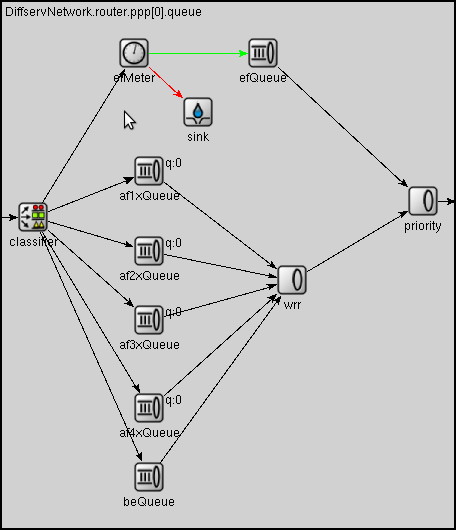
\includegraphics[scale=0.7]{figures/DiffservQueue.png}
\end{center}

The incoming packets are first classified according to
their DSCP field. DSCPs other than AFxy and EF are handled
as BE (best effort).

EF packets are stored in a dedicated queue, and served first
when a packet is requested. Because they can preempt the other
queues, the rate of the EF packets should be limited to a fraction
of the bandwith of the link. This is achieved by metering the EF
traffic with a token bucket meter and dropping packets that
does not conform to the traffic profile.

There are other queues for AFx classes and BE. The AFx queues
use RED to implement 3 different drop priorities within the class.
BE packets are stored in a drop tail queue.
Packets from AFxy and BE queues are sheduled by a WRR scheduler,
which ensures that the remaining bandwith is allocated among the classes
according to the specified weights.

\section{Examples}

% mention 'DiffServ examples' feature

\subsection{Simple domain example}

The \ffilename{examples/diffserv/simple\_} directory contains a
simple demonstration of Diffserv QoS capabilities.

\begin{center}
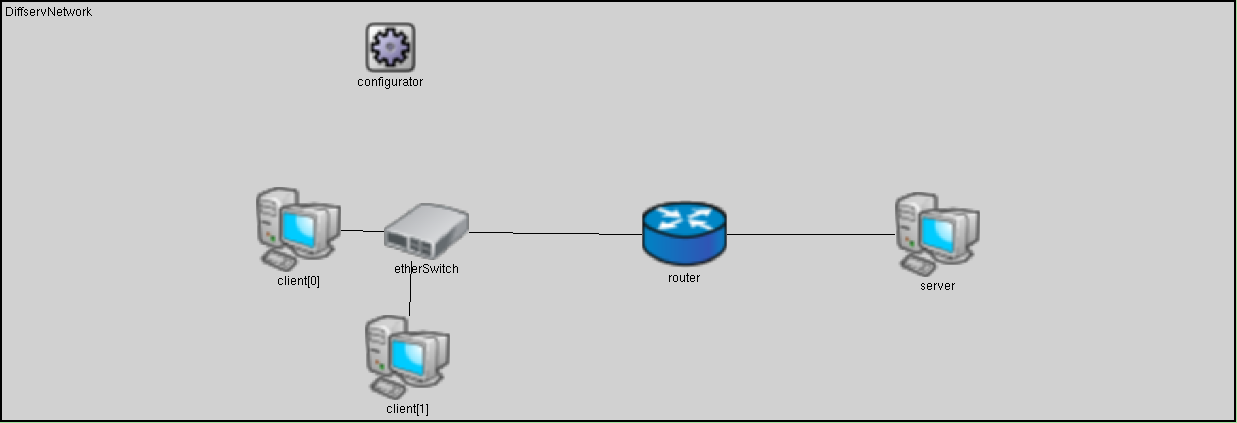
\includegraphics[scale=0.3]{figures/SimpleDiffservNetwork.png}
\end{center}

The network contains a router with an 10Mbps Ethernet interface and a
128kbps dialup link to a server. Clients are configured to generate
high traffic, that causes congestion at the router PPP interface.
One of the clients sends VoIP packets to the server.

With the \ttt{VoIP\_WithoutQoS} configuration, the queue in the router PPP interface
will be overloaded and packets are dropped randomly.

With the \ttt{VoIP\_WithPolicing} configuration, the VoIP traffic is classified as EF
traffic and the necessary bandwidth is allocated for it. The traffic conditioning
is configured so, that packets generated by the other clients are dropped if they
exceed the enabled rate.

With the \ttt{VoIP\_WithPolicingAndQueuing} configuration, the VoIP traffic is classified as EF
traffic and the necessary bandwidth is allocated for it. The router's queue is configured
so that EF packets are prioritized over other packets, so lower delays are expected.

After running these configuration you can see the statistics by opening the
VoIP.anf file, or can hear the difference by comparing the recorded .wav files
in the results directory.

\subsection{One domain example}

The \ffilename{examples/diffserv/onedomain} directory contains
a network in which the routers constitute a single DiffServ domain.
Several experiments are performed on this network, that demonstrates
the resource allocation, and flow isolation capabilities of DiffServ
network compared to the Best Effort service. It also shows the
behavior of the different forwarding classes. These experiments
reproduce the results obtained by an NS3 DiffServ implementation
(\cite{Sanjay2010}).

The network composed of 8 hosts and 6 routers.
Hosts are connected to the routers by 100Mbps Ethernet links. The
routers are connected by PPP lines with lower datarates.
Traffic policing performed at the Ethernet interface of the edge
routers (\ttt{R0},\ttt{R1},\ttt{R4},\ttt{R5}). By changing
the queue module of the PPP interfaces, diverse per-hop behaviors
can be instrumented.

\begin{center}
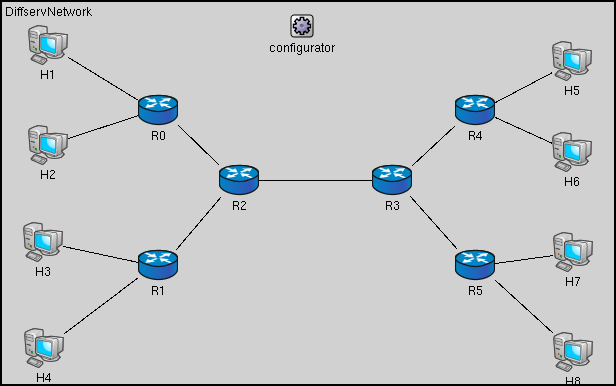
\includegraphics[scale=0.5]{figures/OneDomainDiffservNetwork.png}
\end{center}

Traffic flows from hosts \ttt{H1-H4} to hosts \ttt{H5-H8}. The source hosts
configured to send voice and video data to the destinations hosts. The voice
is sent by an \nedtype{UDPBacisBurst} application, with mean burst duration
352ms, and mean sleep duration 650ms; this mirrors the talk/listen phases
of a phone call. 172 bytes long packets (160 byte data + 12 byte RTP header)
are sent in every 20ms in the burst phase. Considering the IP+UDP overhead,
this results a 80kbps peek rate, and approximately 28kbps avarege rate for
the voice traffic. The video streaming application is modeled by a ~100kbps
CBR traffic, 500 bytes are sent in every 40ms by an \nedtype{UDPBasicApp}
application.

Traffic policing performed at the Ethernet interfaces of the edge routers
(\ttt{R0},\ttt{R1},\ttt{R4},\ttt{R5}). For this purpose a traffic conditioner
is added to the ingress data path of the Ethernet interfaces. The necessary
forwarding behaviours are implemented by changing the external queue module
of the PPP interfaces of routers.

The following sections describe four experiments in detail. The experiments
are numbered from 1 to 5, but 4 is omitted, to keep it consistent with the
numbering in \cite{Sanjay2010}.
The ini file define the configurations for each experiment. Configurations
named \ttt{ExpXY} (where X and Y are digits) belong to Experiment X.
After running each configuration, result can be evaluated by executing
the \ffilename{ExperimentX.R} file with the
\href{http://www.r-project.org}{R statistical program}.

\subsubsection*{Experiment 1}

This experiment shows how the resources of a network can be allocated
to different forwarding classes, and also demontrates the effect of
these allocation on the quality of the service.

In configurations \ttt{Exp11-Exp15}, the traffic from hosts \ttt{H1-H4}
are marked with different AFx1 classes at the edge routers. These
forwarding classes are implemented by PPP queues using a WRR scheduler.
The weights of the different forwarding classes are changed from the most
polarized 7/6/5/4 to the least polarized 1/1/1/1. In the \ttt{Exp16}
configuration, packets of the \ttt{H4} host are classified as EF, so
they have higher priority at forwarding. The last configuration
(\ttt{Exp17}), describing a Best Effort network, serves as a reference
point for other measurements.

Results shows that packets that belong to different AFxy forwarding classes get
different treatments, and the differences are larger when the variance
of the weights is larger. It also can be observed that EF packets
receives much better treatment than others: they have no packet loss,
and have a very low delay.

\subsubsection*{Experiment 2}

This experiment shows how the different drop precedencies of the AFxy
forwarding classes can be implemented by RED queueing. In configurations
\ttt{Exp21-Exp24}, hosts \ttt{H1-H3} sends the normal voice and video
traffic, while \ttt{H4} sends only CBR traffic whose rate changes
from 10kbps to 100kpbs in 10kpbs (so there is 10 measurement for each
configuration). Packets from \ttt{H1-H3} are marked with
increasing drop priority (i.e. \ttt{H1} traffic is forwarded as AF11,
\ttt{H2} as AF12, and \ttt{H3} as AF13). The forwarding treatment
of \ttt{H4} traffic is changing in the different
configurations: AF11 in \ttt{Exp21}, AF12 in \ttt{Exp22}, and
AF13 in \ttt{Exp23}. The \ttt{Exp24} configuration shows the behavior
of a Best Effort network under the same traffic.

The plots shows that in the DiffServ network, there is no loss of
AF11 traffic, and AF12 traffic loss is very low. The average queue
length is lower in \ttt{Exp23}, because the red packets are dropped
more likely.

\subsubsection*{Experiment 3}

This experiment tests bandwidth utilization and flow isolation.
Only hosts \ttt{H1} and \ttt{H2} generate traffic. \ttt{H1} has
an extra \nedtype{UDPBasicApp} application, that generates a CBR
traffic in addition to the voice and video streams. The rate of
this extra traffic varies from 10kbps to 50kbps in 10kpbs steps
in different measurements. Because the PPP links have only
300kbps datarate, the link between \ttt{R2} and \ttt{R3} is
congested when the extra traffic is high enough.

With the first configuration (\ttt{Exp31}), both traffic policing
and DiffServ queues are used. Traffic is metered at the egde routers
by a token bucket meter. Packets whose rate is below 150kbps
marked as AF11, the excess traffic is marked as AF12. RED queues
in the network are configured so, that AF12 packets are dropped
more aggressively than AF11 packets.

With the second configuration (\ttt{Exp32}), only traffic policing
is used. Packets whose rate exceeding the allowed 150kbps limit
are dropped at the boundary of the domain. There is no differentiated
forwarding treatment of packets inside the domain. Each packet goes
to the same queue in the PPP interfaces of routers. They are simple
drop tail queues with 200 frames capacity.

The third configuration describes a Best Effort network.
There is not traffic policing, and the PPP interfaces contain
drop tail queues having buffer space for 200 frames.

As it is expected, the bandwith utilization is high in the first
and third case, but lower in the second case. On the other hand,
the Best Effort network does not provide the same flow isolation
as the DiffServ network. In the third case the well-behaving
\ttt{H3} node suffers from the extra traffic generated by \ttt{H1}.

\subsubsection*{Experiment 5}

This experiment compares a DiffServ network and a Best Effort network.
In the DiffServ network, all voice traffic is marked with EF class
at the edge routers. The video traffic originating from \ttt{H1} and
\ttt{H3} are marked with AF11, while video traffic from \ttt{H2} and
\ttt{H4} are marked with AF21. Routers contain DiffServQueue that
implements the EF and AFxy forwarding classes with priority queueing,
and weighted round-robin queueing. The weight of AF11 is a bit larger,
than the weight of AF21, so hosts \ttt{H1} and \ttt{H3} gets better
services. The queues contain a 100 frame buffer capacity for each forwarding
class.

In the Best Effort network each PPP queue is a \nedtype{DropTailQueue}.
The queue capacities are 200 frames, to keep the buffer space equal to
the DiffServ case.

In the DiffServ network, there is no loss of voice packets. Losses
of video packets are smaller for \ttt{H1} and \ttt{H3} hosts, and
higher for \ttt{H2} and \ttt{H4} than in a Best Effort network.
This is expected, because DiffServ cannot increase the available
resources, it only distributes them differently. It can also be
observed, that the delay of voice packets are much smaller in the
DiffServ network, so it can provide the necessary services for
VoIP applications, while a Best Effort network can not.

\subsection*{Multiple domains example}

This example describes a real-world scenario, and shows how
the SLAs can be implemented with the components offered by INET.

%%% Local Variables:
%%% mode: latex
%%% TeX-master: "usman"
%%% End:



\cleardoublepage

\chapter{The MPLS Models}
\label{cha:mpls}

TODO how to set up/tear down label switched paths; etc.

%%% Local Variables:
%%% mode: latex
%%% TeX-master: "usman"
%%% End:



\cleardoublepage

\ifdraft TODO
\chapter{Applications}
\label{cha:apps}


\ifdraft TODO
\section{Overview}

This chapter describes application models and traffic generators.

Blah blah blah
\fi


%%% Local Variables:
%%% mode: latex
%%% TeX-master: "usman"
%%% End:


\cleardoublepage
\fi

\chapter{History}
\label{cha:History}

\section{IPSuite to INET Framework (2000-2006)}

The predecessor of the INET framework was written by Klaus
Wehrle, Jochen Reber, Dirk Holzhausen, Volker Boehm, Verena Kahmann,
Ulrich Kaage and others at the University of Karlsruhe during 2000-2001,
under the name IPSuite.

The MPLS, LDP and RSVP-TE models were built as an add-on to IPSuite
during 2003 by Xuan Thang Nguyen (Xuan.T.Nguyen@uts.edu.au) and other
students at the University of Technology, Sydney under supervision of
Dr Robin Brown. The package consisted of around 10,000 LOCs, and was
published at http://charlie.it.uts.edu.au/~tkaphan/xtn/capstone (now
unavailable).

After a period of IPSuite being unmaintained, Andras Varga took over
the development in July 2003. Through a series of snapshot releases in
2003-2004, modules got completely reorganized, documented, and many of them
rewritten from scratch. The MPLS models (including RSVP-TE, LDP, etc)
also got refactored and merged into the codebase.

During 2004, Andras added a new, modular and extensible TCP implementation,
application models, Ethernet implementation and an all-in-one IP model
to replace the earlier, modularized one.

The package was renamed INET Framework in October 2004.

Support for wireless and mobile networks got added during summer 2005
by using code from the Mobility Framework.

The MPLS models (including LDP and RSVP-TE) got revised and mostly
rewritten from scratch by Vojta Janota in the first half of 2005
for his diploma thesis. After further refinements by Vojta, the new code
got merged into the INET CVS in fall 2005, and got eventually released
in the March 2006 INET snapshot.

The OSPFv2 model was created by Andras Babos during 2004 for his diploma
thesis which was submitted early 2005. This work was sponsored by Andras Varga,
using revenues from commercial OMNEST licenses. After several refinements and fixes,
the code got merged into the INET Framework in 2005, and became part of the
March 2006 INET snapshot.

The Quagga routing daemon was ported into the INET Framework also by Vojta
Janota. This work was also sponsored by Andras Varga. During fall 2005 and
the months after, ripd and ospfd were ported, and the methodology of porting
was refined. Further Quagga daemons still remain to be ported.

Based on experience from the IPv6Suite (from Ahmet Sekercioglu's group at
CTIE, Monash University, Melbourne) and IPv6SuiteWithINET (Andras's effort
to refactor IPv6Suite and merge it with INET early 2005), Wei Yang Ng
(Monash Uni) implemented a new IPv6 model from scratch for the
INET Framework in 2005 for his diploma thesis, under guidance from Andras
who was visiting Monash between February and June 2005. This IPv6 model
got first included in the July 2005 INET snapshot, and gradually refined
afterwards.

The SCTP implementation was contributed by Michael Tuexen, Irene Ruengeler
and Thomas Dreibholz

Support for Sam Jensen's Network Simulation Cradle,
which makes real-world TCP stacks available in simulations was added
by Zoltan Bojthe in 2010.

TCP SACK and New Reno implementation was contributed by Thomas Reschka.

Several other people have contributed to the INET Framework by providing
feedback, reporting bugs, suggesting features and contributing patches;
I'd like to acknowledge their help here as well.



%%% Local Variables:
%%% mode: latex
%%% TeX-master: "usman"
%%% End:


\cleardoublepage

\bibliographystyle{alpha}
\bibliography{inet-manual}


%% no need for the following since 'tocbibind' package
%% \phantomsection
%% \addcontentsline{toc}{chapter}{\indexname}
\printindex

\end{document}

%%% Local Variables:
%%% mode: latex
%%% TeX-master: t
%%% End:
